% Chapter 2: ARMA Models
% Harvard-quality academic presentation
% Bachelor program, Bucharest University of Economic Studies

\documentclass[9pt, aspectratio=169, t]{beamer}

% Ensure content fits on slides
\setbeamersize{text margin left=8mm, text margin right=8mm}

%=============================================================================
% THEME AND STYLE CONFIGURATION
%=============================================================================
\usetheme{default}
% Using default theme for clean header/footer control

% Color Palette (matching Redispatch PDF)
\definecolor{MainBlue}{RGB}{26, 58, 110}
\definecolor{AccentBlue}{RGB}{26, 58, 110}
\definecolor{IDAred}{RGB}{205, 0, 0}
\definecolor{DarkGray}{RGB}{51, 51, 51}
\definecolor{MediumGray}{RGB}{128, 128, 128}
\definecolor{LightGray}{RGB}{248, 248, 248}
\definecolor{VeryLightGray}{RGB}{235, 235, 235}
\definecolor{KeynoteGray}{RGB}{218, 218, 218}
\definecolor{SectionGray}{RGB}{120, 120, 120}
\definecolor{FooterGray}{RGB}{100, 100, 100}
\definecolor{Crimson}{RGB}{220, 53, 69}
\definecolor{Forest}{RGB}{46, 125, 50}
\definecolor{Amber}{RGB}{181, 133, 63}
\definecolor{Orange}{RGB}{230, 126, 34}
\definecolor{Purple}{RGB}{142, 68, 173}

% Gradient background (exact Keynote 315° gradient: white to RGB 218,218,218)
\setbeamertemplate{background}{%
    \begin{tikzpicture}[remember picture, overlay]
        \shade[shading=axis, shading angle=315,
        top color=white, bottom color=KeynoteGray]
        (current page.south west) rectangle (current page.north east);
    \end{tikzpicture}%
}
% Fallback solid color for compatibility
\setbeamercolor{background canvas}{bg=}

\setbeamercolor{palette primary}{bg=MainBlue, fg=white}
\setbeamercolor{palette secondary}{bg=MainBlue!85, fg=white}
\setbeamercolor{palette tertiary}{bg=MainBlue!70, fg=white}
\setbeamercolor{structure}{fg=MainBlue}
\setbeamercolor{title}{fg=IDAred}
\setbeamercolor{frametitle}{fg=IDAred, bg=}
\setbeamercolor{block title}{bg=MainBlue, fg=white}
\setbeamercolor{block body}{bg=VeryLightGray, fg=DarkGray}
\setbeamercolor{block title alerted}{bg=Crimson, fg=white}
\setbeamercolor{block body alerted}{bg=Crimson!8, fg=DarkGray}
\setbeamercolor{block title example}{bg=Forest, fg=white}
\setbeamercolor{block body example}{bg=Forest!8, fg=DarkGray}
\setbeamercolor{item}{fg=MainBlue}

% Footer colors (override Madrid theme blue)
\setbeamercolor{author in head/foot}{fg=FooterGray, bg=}
\setbeamercolor{title in head/foot}{fg=FooterGray, bg=}
\setbeamercolor{date in head/foot}{fg=FooterGray, bg=}
\setbeamercolor{section in head/foot}{fg=FooterGray, bg=}
\setbeamercolor{subsection in head/foot}{fg=FooterGray, bg=}

% Bullet styles (apply everywhere including blocks)
\setbeamertemplate{itemize item}{\color{MainBlue}$\boxdot$}
\setbeamertemplate{itemize subitem}{\color{MainBlue}$\blacktriangleright$}
\setbeamertemplate{itemize subsubitem}{\color{MainBlue}\tiny$\bullet$}
\setbeamertemplate{itemize/enumerate body begin}{\normalsize}
\setbeamertemplate{itemize/enumerate subbody begin}{\normalsize}

% Item spacing - compact style
\setlength{\leftmargini}{10pt}       % Level 1: minimal indent
\setlength{\leftmarginii}{10pt}      % Level 2: minimal additional indent
% Compact list spacing (zero extra space before/after lists in blocks)
\makeatletter
\def\@listi{\leftmargin\leftmargini \topsep 0pt \parsep 0pt \itemsep 0pt}
\def\@listii{\leftmargin\leftmarginii \topsep 0pt \parsep 0pt \itemsep 0pt}
\makeatother

\setbeamertemplate{navigation symbols}{}

%=============================================================================
% CUSTOM HEADLINE
%=============================================================================
\setbeamertemplate{headline}{%
    \vskip10pt%
    \hbox to \paperwidth{%
        \hskip0.5cm%
        {\small\color{FooterGray}\renewcommand{\hyperlink}[2]{##2}\insertsectionhead}%
        \hfill%
        \textcolor{FooterGray}{\small\insertframenumber}%
        \hskip0.5cm%
    }%
    \vskip4pt%
    {\color{FooterGray}\hrule height 0.4pt}%
}

%=============================================================================
% CUSTOM FOOTER
%=============================================================================
\usepackage{fontawesome5}

\setbeamertemplate{footline}{%
    {\color{FooterGray}\hrule height 0.4pt}%
    \vskip4pt%
    \hbox to \paperwidth{%
        \hskip0.5cm%
        \textcolor{FooterGray}{\small Time Series Analysis and Forecasting}%
        \hfill%
        \raisebox{-0.1em}{%
            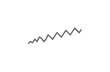
\begin{tikzpicture}[x=0.08em, y=0.08em, line width=0.4pt]
                \draw[FooterGray] (0,3) -- (1,4) -- (2,3.5) -- (3,5) -- (4,4) -- (5,6) -- (6,5.5) -- (7,4) -- (8,5) -- (9,7) -- (10,6) -- (11,5) -- (12,6.5) -- (13,8) -- (14,7) -- (15,6) -- (16,7.5) -- (17,9) -- (18,8) -- (19,7) -- (20,8.5) -- (21,10) -- (22,9) -- (23,8) -- (24,9.5);
            \end{tikzpicture}%
        }%
        \hskip0.5cm%
    }%
    \vskip6pt%
}

%=============================================================================
% PACKAGES
%=============================================================================
\usepackage[utf8]{inputenc}
\usepackage[T1]{fontenc}
\usepackage{amsmath, amssymb, amsthm}
\usepackage{mathtools}
\usepackage{bm}
\usepackage{tikz}
\usetikzlibrary{arrows.meta, positioning, shapes, calc, decorations.pathreplacing, shadings}
\usepackage{booktabs}
\usepackage{multirow}
\usepackage{array}
\usepackage{graphicx}
\usepackage{hyperref}
\usepackage{colortbl}
\hypersetup{colorlinks=true, linkcolor=MainBlue, urlcolor=MainBlue}
\graphicspath{{../../logos/}{../../charts/}}
\hfuzz=2pt  % Suppress tiny overfull warnings (<2pt)
\vfuzz=2pt  % Suppress tiny vertical overfull warnings (<2pt)

%=============================================================================
% QUANTLET COMMAND
%=============================================================================
\newcommand{\quantlet}[2]{%
    \hfill\href{#2}{%
        \raisebox{-0.15em}{\includegraphics[height=0.7em]{ql_logo.png}}%
        \textcolor{MainBlue}{\tiny\ #1}%
    }%
}

%=============================================================================
% CUSTOM TITLE PAGE
%=============================================================================
\defbeamertemplate*{title page}{hybrid}[1][]
{
    \vspace{0.2cm}
    % Logo row - top header (with clickable links)
    \begin{center}
        \href{https://www.ase.ro}{\includegraphics[height=1.0cm]{ase_logo.png}}\hspace{0.3cm}%
        \href{https://theida.net}{\includegraphics[height=1.0cm]{ida_logo.png}}\hspace{0.3cm}%
        \href{https://blockchain-research-center.com}{\includegraphics[height=1.0cm]{brc_logo.png}}\hspace{0.3cm}%
        \href{https://www.ai4efin.ase.ro}{\includegraphics[height=1.0cm]{ai4efin_logo.png}}\hspace{0.3cm}%
        \href{https://ipe.ro/new}{\includegraphics[height=1.0cm]{acad_logo.png}}\hspace{0.3cm}%
        \href{https://www.digital-finance-msca.com}{\includegraphics[height=1.0cm]{msca_logo.png}}%
    \end{center}

    \vspace{0.6cm}

    % Main title with Q logos on sides (with clickable links)
    \begin{center}
        \begin{minipage}{0.1\textwidth}
            \centering
            \href{https://quantlet.com}{\includegraphics[height=1.1cm]{ql_logo.png}}
        \end{minipage}%
        \begin{minipage}{0.78\textwidth}
            \centering
            {\LARGE\bfseries\usebeamercolor[fg]{title}\inserttitle}

            \vspace{0.3cm}

            {\usebeamerfont{subtitle}\usebeamercolor[fg]{title}\insertsubtitle}
        \end{minipage}%
        \begin{minipage}{0.1\textwidth}
            \centering
            \href{https://quantinar.com}{\includegraphics[height=1.1cm]{qr_logo.png}}
        \end{minipage}
    \end{center}

    \vspace{0.6cm}

    % Authors (left-aligned)
    \hspace{0.5cm}{\usebeamerfont{author}\insertauthor}

    \vspace{0.3cm}

    % Institute/Affiliations (left-aligned)
    \hspace{0.5cm}\begin{minipage}[t]{0.9\textwidth}
        \raggedright\small\insertinstitute
    \end{minipage}
}

%=============================================================================
% THEOREM ENVIRONMENTS
%=============================================================================
\theoremstyle{definition}
\setbeamertemplate{theorems}[numbered]
\newtheorem{defn}{Definition}
\newtheorem{thm}{Theorem}
\newtheorem{prop}{Proposition}
\newtheorem{rmk}{Remark}

%=============================================================================
% CUSTOM COMMANDS
%=============================================================================
\newcommand{\E}{\mathbb{E}}
\newcommand{\Var}{\text{Var}}
\newcommand{\Cov}{\text{Cov}}
\newcommand{\Corr}{\text{Corr}}
\newcommand{\R}{\mathbb{R}}
\newcommand{\N}{\mathbb{N}}
\newcommand{\Z}{\mathbb{Z}}
\newcommand{\B}{\mathbf{B}}
\newcommand{\imark}{\textcolor{MainBlue}{\textbullet}}
\newcommand{\RMSE}{\text{RMSE}}
\newcommand{\MAE}{\text{MAE}}
\newcommand{\MAPE}{\text{MAPE}}

%=============================================================================
% TITLE INFORMATION
%=============================================================================
\title[Time Series Analysis]{Time Series Analysis and Forecasting}
\subtitle{Chapter 2: ARMA Models}
\author[D.T. Pele]{Daniel Traian PELE}
\institute{Bucharest University of Economic Studies\\
IDA Institute Digital Assets\\
Blockchain Research Center\\
AI4EFin Artificial Intelligence for Energy Finance\\
Romanian Academy, Institute for Economic Forecasting\\
MSCA Digital Finance}
\date{}

\begin{document}

% Title page (no header/footer)
{
\setbeamertemplate{headline}{}
\setbeamertemplate{footline}{}
\begin{frame}
    \titlepage
\end{frame}
}

%=============================================================================
% LEARNING OBJECTIVES
%=============================================================================
\begin{frame}{Learning Objectives}
    \begin{block}{By the end of this chapter, you will be able to:}
    \begin{enumerate}\setlength{\itemsep}{0pt}
        \item[\textcolor{MainBlue}{\textbf{1.}}] \textbf{Define} and simulate AR($p$), MA($q$), and ARMA($p,q$) processes
        \item[\textcolor{MainBlue}{\textbf{2.}}] \textbf{Verify} stationarity and invertibility conditions
        \item[\textcolor{MainBlue}{\textbf{3.}}] \textbf{Identify} orders $p$ and $q$ through ACF/PACF analysis
        \item[\textcolor{MainBlue}{\textbf{4.}}] \textbf{Estimate} parameters via Yule-Walker, MLE, and information criteria (AIC, BIC)
        \item[\textcolor{MainBlue}{\textbf{5.}}] \textbf{Diagnose} the model through residual analysis and the Ljung-Box test
        \item[\textcolor{MainBlue}{\textbf{6.}}] \textbf{Forecast} using ARMA models with confidence intervals
        \item[\textcolor{MainBlue}{\textbf{7.}}] \textbf{Apply} the Box-Jenkins methodology to real data (sunspots)
    \end{enumerate}
    \end{block}
\end{frame}

%=============================================================================
% TABLE OF CONTENTS
%=============================================================================
\begin{frame}{Chapter Structure}
    \setbeamertemplate{section in toc}{\color{MainBlue}$\boxdot$~\inserttocsection}
    {\footnotesize
    \begin{columns}[T]
        \begin{column}{0.48\textwidth}
            \tableofcontents[sections={1-7}, hideallsubsections]
        \end{column}
        \begin{column}{0.48\textwidth}
            \tableofcontents[sections={8-13}, hideallsubsections]
        \end{column}
    \end{columns}
    }
\end{frame}

%=============================================================================
% MOTIVATION
%=============================================================================
\section{Motivation}

\begin{frame}{Why ARMA Models?}
    \vspace{-0.3cm}
    \begin{center}
        \includegraphics[width=0.92\textwidth, height=0.62\textheight, keepaspectratio]{ch2_motivation_stationary.pdf}
    \end{center}
    \vspace{-0.2cm}
    {\footnotesize
    \begin{itemize}
        \item \textbf{AR processes}: Current value depends on past values $\succ$ mean-reverting behavior
        \item \textbf{MA processes}: Current value depends on past shocks $\succ$ short memory
        \item \textbf{ARMA}: Combines both mechanisms for flexible modeling
    \end{itemize}
    }
    \quantlet{TSA\_ch2\_motivation}{https://github.com/QuantLet/TSA/tree/main/TSA_ch2/TSA_ch2_motivation}
\end{frame}

\begin{frame}{Model Identification Through ACF Patterns}
    \vspace{-0.3cm}
    \begin{center}
        \includegraphics[width=0.92\textwidth, height=0.52\textheight, keepaspectratio]{ch2_motivation_acf.pdf}
    \end{center}
    \vspace{-0.2cm}
    {\footnotesize
    \begin{exampleblock}{ACF Reflects Model Structure}
        \begin{itemize}\setlength{\itemsep}{0pt}
            \item \textbf{Distinct patterns}: AR: exponential decay; MA: sharp cutoff; ARMA: mixed decay
            \item \textbf{Identification}: Visual analysis of ACF/PACF guides the selection of orders $p$ and $q$
        \end{itemize}
    \end{exampleblock}
    }
    \quantlet{TSA\_ch2\_motivation}{https://github.com/QuantLet/TSA/tree/main/TSA_ch2/TSA_ch2_motivation}
\end{frame}

%=============================================================================
% SECTION 1: INTRODUCTION AND THE LAG OPERATOR
%=============================================================================
\section{Introduction and the Lag Operator}

\begin{frame}{Recap: Stationarity}
    \vspace{-0.3cm}
    \small
    \begin{block}{From Chapter 1}
        \begin{itemize}\setlength{\itemsep}{0pt}
            \item A process $\{X_t\}$ is \textbf{weakly stationary} if:
            \begin{enumerate}\setlength{\itemsep}{0pt}
                \item $\E[X_t] = \mu$ (constant mean)
                \item $\Var(X_t) = \sigma^2 < \infty$ (constant, finite variance)
                \item $\Cov(X_t, X_{t+h}) = \gamma(h)$ (covariance depends only on lag $h$)
            \end{enumerate}
        \end{itemize}
    \end{block}
    \vspace{-0.2cm}
    \begin{exampleblock}{Why Stationarity Matters for ARMA}
        \begin{itemize}\setlength{\itemsep}{0pt}
            \item \textcolor{Forest}{ARMA models assume stationarity}
            \begin{itemize}
                \item Parameters remain stable over time
                \item Autocorrelation structure is maintained
            \end{itemize}
            \item \textcolor{Crimson}{Non-stationary data} $\succ$ difference first (ARIMA, Ch. 3)
        \end{itemize}
    \end{exampleblock}
    \vspace{-0.2cm}
    \begin{alertblock}{Chapter Objective}
        \begin{itemize}\setlength{\itemsep}{0pt}
            \item Parametric models for stationary series $\succ$ combining dependence on past observations (AR) with the influence of random shocks (MA)
        \end{itemize}
    \end{alertblock}
\end{frame}

\begin{frame}{The Lag Operator (Backshift Operator)}
    \vspace{-0.2cm}
    \begin{defn}[Lag Operator]
        \begin{itemize}\setlength{\itemsep}{0pt}
            \item The \textbf{lag operator} $L$ (or backshift operator $B$) shifts a time series back by one period: $L X_t = X_{t-1}$
        \end{itemize}
    \end{defn}
    \vspace{-0.2cm}
    \begin{block}{Properties}
        \begin{itemize}\setlength{\itemsep}{0pt}
            \item $L^k X_t = X_{t-k}$ (shift back by $k$ periods)
            \item $L^0 X_t = X_t$ (identity)
            \item $(1-L)X_t = X_t - X_{t-1} = \Delta X_t$ (first difference)
            \item $(1-L)^d X_t = \Delta^d X_t$ (difference of order $d$)
        \end{itemize}
    \end{block}
    \vspace{-0.2cm}
    \begin{exampleblock}{Lag Polynomials}
        \begin{itemize}\setlength{\itemsep}{0pt}
            \item \textbf{AR polynomial}: $\phi(L) = 1 - \phi_1 L - \phi_2 L^2 - \cdots - \phi_p L^p$
            \item \textbf{MA polynomial}: $\theta(L) = 1 + \theta_1 L + \theta_2 L^2 + \cdots + \theta_q L^q$
        \end{itemize}
    \end{exampleblock}
    \quantlet{TSA\_ch2\_lag\_operator}{https://github.com/QuantLet/TSA/tree/main/TSA_ch2/TSA_ch2_lag_operator}
\end{frame}

\begin{frame}{The Lag Operator: Visual Illustration}
    \begin{center}
        \includegraphics[width=0.88\textwidth, height=0.62\textheight, keepaspectratio]{lag_operator.pdf}
    \end{center}
    \vspace{-0.2cm}
    {\footnotesize
    \begin{block}{Role of the Lag Operator}
        \begin{itemize}\setlength{\itemsep}{0pt}
            \item \textbf{Notation foundation}: Enables compact writing of difference equations
            \item \textbf{Utility}: Facilitates algebraic manipulation of ARMA models
        \end{itemize}
    \end{block}
    }
    \quantlet{TSA\_ch2\_lag\_operator}{https://github.com/QuantLet/TSA/tree/main/TSA_ch2/TSA_ch2_lag_operator}
\end{frame}

\begin{frame}{The White Noise Process}
    \vspace{-0.2cm}
    \begin{defn}[White Noise]
        \begin{itemize}\setlength{\itemsep}{0pt}
            \item A process $\{\varepsilon_t\}$ is \textbf{white noise}, denoted $\varepsilon_t \sim WN(0, \sigma^2)$, if:
            \begin{enumerate}
                \item $\E[\varepsilon_t] = 0$ for all $t$
                \item $\Var(\varepsilon_t) = \sigma^2$ for all $t$
                \item $\Cov(\varepsilon_t, \varepsilon_s) = 0$ for all $t \neq s$
            \end{enumerate}
        \end{itemize}
    \end{defn}
    \vspace{-0.2cm}
    {\footnotesize
    \begin{block}{Properties}
        \begin{itemize}\setlength{\itemsep}{0pt}
            \item \textbf{Building block}: White noise underlies all ARMA models
            \item \textbf{ACF}: $\rho(0) = 1$, $\rho(h) = 0$ for $h \neq 0$; PACF: same pattern
            \item \textbf{Gaussian white noise}: $\varepsilon_t \sim N(0, \sigma^2)$ i.i.d.
            \item \textbf{Unpredictable}: White noise is \textit{not} predictable $\succ$ it is purely random
        \end{itemize}
    \end{block}
    }
\end{frame}

\begin{frame}{White Noise: Visual Illustration}
    \vspace{-0.2cm}
    \begin{columns}[T]
        \begin{column}{0.32\textwidth}
            \vspace{0.3cm}
            {\footnotesize
            \begin{block}{Key Characteristics}
                \begin{itemize}\setlength{\itemsep}{2pt}
                    \item \textbf{Top}: Random fluctuations, no patterns, constant variance
                    \item \textbf{Bottom}: ACF only a spike at lag 0; others within significance bounds $\succ$ no linear dependence
                \end{itemize}
            \end{block}
            }
            \vspace{0.2cm}
            \quantlet{TSA\_ch2\_white\_noise}{https://github.com/QuantLet/TSA/tree/main/TSA_ch2/TSA_ch2_white_noise}
        \end{column}
        \begin{column}{0.66\textwidth}
            \includegraphics[width=\textwidth, height=0.78\textheight, keepaspectratio]{ch2_white_noise.pdf}
        \end{column}
    \end{columns}
\end{frame}

%=============================================================================
% SECTION 2: AR MODELS
%=============================================================================
\section{Autoregressive (AR) Models}

\begin{frame}{The AR(1) Model: Definition}
    \vspace{-0.2cm}
    \begin{defn}[AR(1) Process]
        \begin{itemize}\setlength{\itemsep}{0pt}
            \item An \textbf{autoregressive process of order 1} is: $X_t = c + \phi X_{t-1} + \varepsilon_t$
            \item $\varepsilon_t \sim WN(0, \sigma^2)$ and $|\phi| < 1$ for stationarity
        \end{itemize}
    \end{defn}
    \vspace{-0.2cm}
    \begin{columns}[T]
        \begin{column}{0.48\textwidth}
        \begin{block}{Interpretation}
            \begin{itemize}\setlength{\itemsep}{0pt}
                \item $c$: constant (intercept)
                \item $\phi$: autoregressive coefficient
                \begin{itemize}
                    \item Measures the persistence of the series
                \end{itemize}
                \item $\varepsilon_t$: innovation (shock)
            \end{itemize}
        \end{block}
        \end{column}
        \begin{column}{0.48\textwidth}
        \begin{exampleblock}{Lag Operator Notation}
            \begin{itemize}\setlength{\itemsep}{0pt}
                \item $(1 - \phi L)X_t = c + \varepsilon_t$
                \item $\phi(L) X_t = c + \varepsilon_t$
                \item $\phi(L) = 1 - \phi L$
            \end{itemize}
        \end{exampleblock}
        \end{column}
    \end{columns}
\end{frame}

\begin{frame}{AR(1): Visual Illustration}
    \begin{center}
        \includegraphics[width=0.95\textwidth, height=0.52\textheight, keepaspectratio]{ch2_def_ar1.pdf}
    \end{center}
    \vspace{-0.2cm}
    {\footnotesize
    \begin{block}{Visual Interpretation}
        \begin{itemize}\setlength{\itemsep}{0pt}
            \item \textbf{Positive $\phi$}: Persistent fluctuations, gradual mean reversion
            \item \textbf{Negative $\phi$}: Oscillating behavior, alternating around the mean
            \item Larger $|\phi|$ $\succ$ greater persistence, slower reversion
        \end{itemize}
    \end{block}
    }
    \quantlet{TSA\_ch2\_ar1}{https://github.com/QuantLet/TSA/tree/main/TSA_ch2/TSA_ch2_ar1}
\end{frame}

\begin{frame}{AR(1) Stationarity Condition}
    \vspace{-0.2cm}
    \begin{alertblock}{Necessary and Sufficient Condition: $|\phi| < 1$}
        \begin{itemize}\setlength{\itemsep}{0pt}
            \item The root of the characteristic equation must lie outside the unit circle
        \end{itemize}
    \end{alertblock}
    \vspace{-0.2cm}
    \begin{columns}[T]
        \begin{column}{0.48\textwidth}
        \begin{exampleblock}{\textcolor{Forest}{Stationary ($|\phi| < 1$)}}
            \begin{itemize}\setlength{\itemsep}{0pt}
                \item Shocks diminish over time
                \begin{itemize}
                    \item Process reverts to the mean
                    \item Finite, stable variance
                \end{itemize}
            \end{itemize}
        \end{exampleblock}
        \end{column}
        \begin{column}{0.48\textwidth}
        \begin{alertblock}{\textcolor{white}{Non-stationary ($|\phi| \geq 1$)}}
            \begin{itemize}\setlength{\itemsep}{0pt}
                \item $|\phi| = 1$: random walk
                \begin{itemize}
                    \item Unit root, variance $\to \infty$
                \end{itemize}
                \item $|\phi| > 1$: explosive process
            \end{itemize}
        \end{alertblock}
        \end{column}
    \end{columns}
    \vspace{-0.2cm}
    \begin{block}{Characteristic Equation}
        \begin{itemize}\setlength{\itemsep}{0pt}
            \item $\phi(z) = 1 - \phi z = 0 \implies z = 1/\phi$
            \item Stationarity $\Leftrightarrow$ root outside the unit circle ($|z|>1$)
        \end{itemize}
    \end{block}
\end{frame}

\begin{frame}{AR(1) Properties}
    \vspace{-0.2cm}
    \begin{block}{Stationary AR(1) with $|\phi| < 1$}
    \begin{itemize}\setlength{\itemsep}{0pt}
    \item Moment properties:
    \end{itemize}
    \vspace{-0.2cm}
    \begin{columns}[T]
        \begin{column}{0.48\textwidth}
        {\small \textbf{Mean:} $\mu = \E[X_t] = \frac{c}{1-\phi}$}

        {\small \textbf{Variance:} $\gamma(0) = \Var(X_t) = \frac{\sigma^2}{1-\phi^2}$}
        \end{column}
        \begin{column}{0.48\textwidth}
        {\small \textbf{Autocovariance:} $\gamma(h) = \frac{\phi^h \sigma^2}{1-\phi^2}$}

        {\small \textbf{Autocorrelation (ACF):} $\rho(h) = \phi^h$}
        \end{column}
    \end{columns}
    \end{block}
    \vspace{-0.2cm}
    \begin{alertblock}{Key Observation}
        \begin{itemize}\setlength{\itemsep}{0pt}
            \item \textbf{AR(1) signature}: ACF decays exponentially with factor $\phi$
            \begin{itemize}
                \item $\phi > 0$: monotone decay towards zero
                \item $\phi < 0$: damped oscillations (alternating signs)
            \end{itemize}
        \end{itemize}
    \end{alertblock}
    \quantlet{TSA\_ch2\_ar1}{https://github.com/QuantLet/TSA/tree/main/TSA_ch2/TSA_ch2_ar1}
\end{frame}

\begin{frame}{Proof: AR(1) Mean}
    \vspace{-0.3cm}
    \begin{block}{Claim}
        \begin{itemize}\setlength{\itemsep}{0pt}
            \item For AR(1): $X_t = c + \phi X_{t-1} + \varepsilon_t$, the mean is $\mu = \frac{c}{1-\phi}$
        \end{itemize}
    \end{block}
    \vspace{-0.3cm}
    {\small
    \begin{exampleblock}{Proof}
        \begin{itemize}\setlength{\itemsep}{0pt}
            \item Take expectations of both sides: $\E[X_t] = c + \phi \E[X_{t-1}] + \E[\varepsilon_t]$
            \item By stationarity, $\E[X_t] = \E[X_{t-1}] = \mu$, and $\E[\varepsilon_t] = 0$: $\mu = c + \phi \mu$
            \item Solving: $\mu - \phi\mu = c \implies \mu(1-\phi) = c \implies \boxed{\mu = \frac{c}{1-\phi}}$
        \end{itemize}
    \end{exampleblock}
    }
    \vspace{-0.2cm}
    \begin{alertblock}{Requirement}
        \begin{itemize}\setlength{\itemsep}{0pt}
            \item \textbf{Necessary condition}: $\phi \neq 1$ for the mean to be defined
            \begin{itemize}
                \item If $\phi = 1$ (unit root), the mean is undefined
                \item The process becomes a random walk (non-stationarity)
            \end{itemize}
        \end{itemize}
    \end{alertblock}
\end{frame}

\begin{frame}{Proof: AR(1) Variance}
    \vspace{-0.3cm}
    \begin{block}{Claim}
        \begin{itemize}\setlength{\itemsep}{0pt}
            \item $\Var(X_t) = \frac{\sigma^2}{1-\phi^2}$
        \end{itemize}
    \end{block}
    \vspace{-0.3cm}
    {\small
    \begin{exampleblock}{Proof}
        \begin{itemize}\setlength{\itemsep}{0pt}
            \item Assume $c=0$. Take the variance of $X_t = \phi X_{t-1} + \varepsilon_t$:
            \item $\Var(X_t) = \phi^2 \Var(X_{t-1}) + \Var(\varepsilon_t) + 2\phi\underbrace{\Cov(X_{t-1}, \varepsilon_t)}_{=0}$
            \item By stationarity, $\Var(X_t) = \Var(X_{t-1}) = \gamma(0)$:
            \item $\gamma(0) = \phi^2 \gamma(0) + \sigma^2 \implies \gamma(0)(1-\phi^2) = \sigma^2 \implies \boxed{\gamma(0) = \frac{\sigma^2}{1-\phi^2}}$
        \end{itemize}
    \end{exampleblock}
    }
    \vspace{-0.2cm}
    \begin{alertblock}{Note}
        \begin{itemize}\setlength{\itemsep}{0pt}
            \item Requires $|\phi| < 1$ for positive variance. When $|\phi| \to 1$, variance $\to \infty$
        \end{itemize}
    \end{alertblock}
\end{frame}

\begin{frame}{Proof: AR(1) Autocorrelation Function}
    \vspace{-0.3cm}
    \begin{block}{Claim: $\rho(h) = \phi^h$ for $h \geq 0$}
        \begin{itemize}\setlength{\itemsep}{0pt}
            \item Find the autocovariance $\gamma(h) = \Cov(X_t, X_{t-h})$
        \end{itemize}
    \end{block}
    \vspace{-0.3cm}
    {\small
    \begin{exampleblock}{Proof}
        \begin{itemize}\setlength{\itemsep}{0pt}
            \item Multiply $X_t = \phi X_{t-1} + \varepsilon_t$ by $X_{t-h}$ and take expectations:
            \item $\E[X_t X_{t-h}] = \phi \E[X_{t-1} X_{t-h}] + \E[\varepsilon_t X_{t-h}]$
            \item For $h \geq 1$: $\E[\varepsilon_t X_{t-h}] = 0$ $\succ$ $\gamma(h) = \phi \gamma(h-1)$
            \item Recursive relation from $\gamma(0)$: $\gamma(1) = \phi\gamma(0)$, $\gamma(2) = \phi^2\gamma(0)$, $\ldots$ $\boxed{\gamma(h) = \phi^h\gamma(0)}$
            \item ACF: $\rho(h) = \frac{\gamma(h)}{\gamma(0)} = \frac{\phi^h\gamma(0)}{\gamma(0)} = \boxed{\phi^h}$
        \end{itemize}
    \end{exampleblock}
    }
\end{frame}

\begin{frame}{AR(1) Variance as a Function of $\phi$}
    \begin{center}
        \includegraphics[width=0.85\textwidth, height=0.58\textheight, keepaspectratio]{ar1_variance.pdf}
    \end{center}
    \vspace{-0.2cm}
    {\footnotesize
    \begin{block}{Observations}
        \begin{itemize}\setlength{\itemsep}{0pt}
            \item As $|\phi| \to 1$, the variance explodes $\succ$ non-stationarity
            \item For $\phi = 0$: $\gamma(0) = \sigma^2$ (white noise); variance increases monotonically with $|\phi|$
        \end{itemize}
    \end{block}
    }
    \quantlet{TSA\_ch2\_ar1}{https://github.com/QuantLet/TSA/tree/main/TSA_ch2/TSA_ch2_ar1}
\end{frame}

\begin{frame}{AR(1) Simulations: Effect of $\phi$}
    \vspace{-0.3cm}
    \begin{center}
        \includegraphics[width=0.82\textwidth, height=0.55\textheight, keepaspectratio]{ch2_ar1_simulations.pdf}
    \end{center}
    \vspace{-0.2cm}
    {\footnotesize
    \begin{block}{Interpretation}
        \begin{itemize}\setlength{\itemsep}{0pt}
            \item Different values of $\phi$ produce distinct behaviors: larger $|\phi|$ $\succ$ more persistence
            \item Positive $\phi$ creates smooth trajectories; negative $\phi$ creates oscillations
            \item As $|\phi| \to 1$, the process approaches non-stationarity
        \end{itemize}
    \end{block}
    }
    \quantlet{TSA\_ch2\_ar1\_simulation}{https://github.com/QuantLet/TSA/tree/main/TSA_ch2/TSA_ch2_ar1_simulation}
\end{frame}

\begin{frame}{Theoretical AR(1) ACF}
    \vspace{-0.2cm}
    \begin{center}
        \includegraphics[width=0.85\textwidth, height=0.58\textheight, keepaspectratio]{ar1_theoretical_acf.pdf}
    \end{center}
    \vspace{-0.2cm}
    {\footnotesize
    \begin{block}{ACF Pattern}
        \begin{itemize}\setlength{\itemsep}{0pt}
            \item \textbf{Formula}: $\rho(h) = \phi^h$ $\succ$ exponential decay
            \item $\phi > 0$: monotone decay; $\phi < 0$: alternating signs
        \end{itemize}
    \end{block}
    }
    \quantlet{TSA\_ch2\_ar1}{https://github.com/QuantLet/TSA/tree/main/TSA_ch2/TSA_ch2_ar1}
\end{frame}

\begin{frame}{Proof: AR(1) Stationarity Condition}
    \vspace{-0.3cm}
    \begin{block}{Claim}
        \begin{itemize}\setlength{\itemsep}{0pt}
            \item AR(1) is stationary if and only if $|\phi| < 1$
        \end{itemize}
    \end{block}
    \vspace{-0.3cm}
    {\small
    \begin{exampleblock}{Proof}
        \begin{itemize}\setlength{\itemsep}{0pt}
            \item Recursive substitution: $X_t = \phi X_{t-1} + \varepsilon_t = \phi(\phi X_{t-2} + \varepsilon_{t-1}) + \varepsilon_t = \cdots$
            \item After $n$ steps: $X_t = \phi^n X_{t-n} + \sum_{j=0}^{n-1}\phi^j\varepsilon_{t-j}$
            \item If $|\phi| < 1$: $\phi^n \to 0$ as $n \to \infty$, so $X_t = \sum_{j=0}^{\infty}\phi^j\varepsilon_{t-j}$
            \item Finite variance: $\Var(X_t) = \sigma^2\sum_{j=0}^{\infty}\phi^{2j} = \frac{\sigma^2}{1-\phi^2} < \infty$ \quad (geometric series)
        \end{itemize}
    \end{exampleblock}
    }
    \vspace{-0.2cm}
    \begin{alertblock}{Conclusion}
        \begin{itemize}\setlength{\itemsep}{0pt}
            \item Converges $\iff |\phi| < 1$. For $|\phi| \geq 1$, the term $\phi^n X_{t-n}$ does not vanish $\Rightarrow$ infinite variance
        \end{itemize}
    \end{alertblock}
\end{frame}

\begin{frame}{AR(1) ACF and PACF: Theory vs Sample}
    \vspace{-0.3cm}
    \begin{center}
        \includegraphics[width=0.82\textwidth, height=0.55\textheight, keepaspectratio]{ch2_ar1_acf_pacf.pdf}
    \end{center}
    \vspace{-0.2cm}
    {\footnotesize
    \begin{block}{Interpretation}
        \begin{itemize}\setlength{\itemsep}{0pt}
            \item \textbf{ACF}: Exponential decay with factor $\phi$; formula: $\rho(h) = \phi^h$
            \item \textbf{PACF}: A single spike at lag 1, then cuts off $\succ$ identifies AR(1)
            \item Sample estimates fluctuate around theoretical values
        \end{itemize}
    \end{block}
    }
    \quantlet{TSA\_ch2\_ar1}{https://github.com/QuantLet/TSA/tree/main/TSA_ch2/TSA_ch2_ar1}
\end{frame}

\begin{frame}{The Partial Autocorrelation Function (PACF)}
    \vspace{-0.3cm}
    \begin{defn}[PACF]
        \begin{itemize}\setlength{\itemsep}{0pt}
            \item The \textbf{partial autocorrelation} of order $k$, denoted $\pi_k$, measures the correlation between $X_t$ and $X_{t-k}$ \textbf{after removing} the linear effects of the intermediate variables $X_{t-1}, \ldots, X_{t-k+1}$
        \end{itemize}
    \end{defn}
    \vspace{-0.3cm}
    {\small
    \begin{columns}[T]
        \begin{column}{0.48\textwidth}
        \begin{block}{Formal Definition}
            \begin{itemize}\setlength{\itemsep}{0pt}
                \item $\pi_1 = \rho(1)$
                \item For $k \geq 2$: $\pi_k$ is the last coefficient in: $X_t = \alpha_1 X_{t-1} + \cdots + \alpha_k X_{t-k} + e_t$
                \item $\pi_k = \alpha_k$ (coefficient of $X_{t-k}$)
            \end{itemize}
        \end{block}
        \end{column}
        \begin{column}{0.48\textwidth}
        \begin{exampleblock}{Computation via Yule-Walker}
            \begin{itemize}\setlength{\itemsep}{0pt}
                \item Solve the Yule-Walker equations of order $k$
                \item $\pi_k$ = last element of the solution vector
            \end{itemize}
        \end{exampleblock}
        \vspace{-0.2cm}
        \begin{alertblock}{Utility}
            \begin{itemize}\setlength{\itemsep}{0pt}
                \item \textbf{Identification}: PACF determines the order $p$ of an AR model
                \begin{itemize}
                    \item PACF cuts off after lag $p$
                \end{itemize}
            \end{itemize}
        \end{alertblock}
        \end{column}
    \end{columns}
    }
\end{frame}

\begin{frame}{AR(1) ACF and PACF Patterns}
    \begin{columns}[T]
        \begin{column}{0.48\textwidth}
        \begin{block}{ACF of AR(1)}
            \begin{itemize}\setlength{\itemsep}{0pt}
                \item Decays exponentially: $\rho(h) = \phi^h$
                \begin{itemize}
                    \item $\phi > 0$: all positive
                    \item $\phi < 0$: alternating signs
                \end{itemize}
            \end{itemize}
        \end{block}
        \end{column}
        \begin{column}{0.48\textwidth}
        \begin{block}{PACF of AR(1)}
            \begin{itemize}\setlength{\itemsep}{0pt}
                \item \textbf{Cuts off after lag 1}
                \begin{itemize}
                    \item $\pi_1 = \phi$, $\pi_k = 0$ for $k > 1$
                \end{itemize}
            \end{itemize}
        \end{block}
        \end{column}
    \end{columns}

    \vspace{0.1cm}
    \begin{center}
    \begin{tabular}{lcc}
        \toprule
        & \textbf{ACF} & \textbf{PACF} \\
        \midrule
        AR(1) & Exponential decay & Cuts off at lag 1 \\
        \bottomrule
    \end{tabular}
    \end{center}

    \vspace{0.1cm}
    \begin{alertblock}{Key Pattern}
        \begin{itemize}\setlength{\itemsep}{0pt}
            \item This is the key identification pattern for AR(1)!
        \end{itemize}
    \end{alertblock}
\end{frame}

\begin{frame}{The AR(p) Model: General Form}
    \vspace{-0.2cm}
    \begin{defn}[AR(p) Process]
        \begin{itemize}\setlength{\itemsep}{0pt}
            \item An \textbf{autoregressive process of order p} is: $X_t = c + \phi_1 X_{t-1} + \phi_2 X_{t-2} + \cdots + \phi_p X_{t-p} + \varepsilon_t$
            \item \textbf{Lag operator}: $\phi(L) X_t = c + \varepsilon_t$, where $\phi(L) = 1 - \phi_1 L - \phi_2 L^2 - \cdots - \phi_p L^p$
        \end{itemize}
    \end{defn}
    \vspace{-0.2cm}
    \begin{block}{Stationarity Condition}
        \begin{itemize}\setlength{\itemsep}{0pt}
            \item All roots of $\phi(z) = 0$ must lie \textbf{outside} the unit circle
            \item Equivalently: all roots have modulus $> 1$
        \end{itemize}
    \end{block}
    \vspace{-0.2cm}
    \begin{exampleblock}{PACF Pattern}
        \begin{itemize}\setlength{\itemsep}{0pt}
            \item PACF cuts off after lag $p$
            \item ACF decays (exponentially or with damped oscillations)
        \end{itemize}
    \end{exampleblock}
\end{frame}

\begin{frame}{AR(p): Visual Illustration}
    \vspace{-0.2cm}
    \begin{center}
        \includegraphics[width=0.92\textwidth, height=0.55\textheight, keepaspectratio]{ch2_def_arp.pdf}
    \end{center}
    \vspace{-0.3cm}
    {\footnotesize
    \begin{block}{Observations}
        \begin{itemize}\setlength{\itemsep}{0pt}
            \item AR(2) can exhibit pseudo-cyclic behavior (complex roots); damped sinusoidal ACF
            \item PACF cuts off after lag 2 $\succ$ key identification pattern
        \end{itemize}
    \end{block}
    }
    \quantlet{TSA\_ch2\_ar2}{https://github.com/QuantLet/TSA/tree/main/TSA_ch2/TSA_ch2_ar2}
\end{frame}

\begin{frame}{AR(2) Stationarity: Unit Circle Visualization}
    \begin{center}
        \includegraphics[width=0.85\textwidth, height=0.49\textheight, keepaspectratio]{unit_circle_stationarity.pdf}
    \end{center}
    \vspace{-0.2cm}
    {\footnotesize
    \begin{block}{Characteristic Polynomial and Unit Circle Condition}
        \begin{itemize}\setlength{\itemsep}{0pt}
            \item \textbf{Characteristic polynomial} of an AR($p$) process: $\phi(z) = 1 - \phi_1 z - \phi_2 z^2 - \cdots - \phi_p z^p$
            \item All roots of $\phi(z) = 0$ must lie \textbf{outside} the unit circle ($|z| > 1$)
            \item Roots on the circle: non-stationary; roots inside: explosive process
        \end{itemize}
    \end{block}
    }
    \quantlet{TSA\_ch2\_stationarity}{https://github.com/QuantLet/TSA/tree/main/TSA_ch2/TSA_ch2_stationarity}
\end{frame}

\begin{frame}{The AR(2) Stationarity Triangle}
    \vspace{-0.3cm}
    \begin{center}
        \includegraphics[width=0.82\textwidth, height=0.55\textheight, keepaspectratio]{ch2_ar2_stationarity.pdf}
    \end{center}
    \vspace{-0.2cm}
    {\footnotesize
    \begin{block}{Stationarity Region}
        \begin{itemize}\setlength{\itemsep}{0pt}
            \item The triangular region defines the stationary AR(2) parameter combinations
            \item \textbf{Boundaries}: $\phi_1 + \phi_2 < 1$, $\phi_2 - \phi_1 < 1$ and $|\phi_2| < 1$
            \item Points outside the region $\succ$ non-stationary or explosive processes
        \end{itemize}
    \end{block}
    }
    \quantlet{TSA\_ch2\_stationarity}{https://github.com/QuantLet/TSA/tree/main/TSA_ch2/TSA_ch2_stationarity}
\end{frame}

\begin{frame}{Characteristic Polynomial Roots}
    \vspace{-0.2cm}
    \begin{center}
        \includegraphics[width=0.88\textwidth, height=0.58\textheight, keepaspectratio]{characteristic_roots.pdf}
    \end{center}
    \vspace{-0.3cm}
    {\footnotesize
    \begin{block}{Types of Roots}
        \begin{itemize}\setlength{\itemsep}{0pt}
            \item \textbf{Real roots}: exponential decay in ACF
            \item \textbf{Complex roots}: damped oscillations (pseudo-cycles)
            \item All roots must lie outside the unit circle
        \end{itemize}
    \end{block}
    }
    \quantlet{TSA\_ch2\_stationarity}{https://github.com/QuantLet/TSA/tree/main/TSA_ch2/TSA_ch2_stationarity}
\end{frame}

\begin{frame}{The AR(2) Model}
    \vspace{-0.2cm}
    \begin{defn}[AR(2) Process]
        \begin{itemize}\setlength{\itemsep}{0pt}
            \item $X_t = c + \phi_1 X_{t-1} + \phi_2 X_{t-2} + \varepsilon_t$
        \end{itemize}
    \end{defn}
    \vspace{-0.2cm}
    \begin{block}{Stationarity Conditions}
        \begin{itemize}\setlength{\itemsep}{0pt}
            \item $\phi_1 + \phi_2 < 1$; \quad $\phi_2 - \phi_1 < 1$; \quad $|\phi_2| < 1$
        \end{itemize}
    \end{block}
    \vspace{-0.2cm}
    \begin{exampleblock}{ACF Behavior}
        \begin{itemize}\setlength{\itemsep}{0pt}
            \item \textbf{Real roots}: mixture of two exponential decays
            \item \textbf{Complex roots}: damped sinusoidal pattern (pseudo-cycles)
            \item \textbf{PACF}: Cuts off after lag 2 ($\pi_k = 0$ for $k > 2$)
        \end{itemize}
    \end{exampleblock}
    \quantlet{TSA\_ch2\_ar2}{https://github.com/QuantLet/TSA/tree/main/TSA_ch2/TSA_ch2_ar2}
\end{frame}

%=============================================================================
% SECTION 3: MA MODELS
%=============================================================================
\section{Moving Average (MA) Models}

\begin{frame}{The MA(1) Model: Definition}
    \vspace{-0.2cm}
    \begin{defn}[MA(1) Process]
        \begin{itemize}\setlength{\itemsep}{0pt}
            \item A \textbf{moving average process of order 1} is: $X_t = \mu + \varepsilon_t + \theta \varepsilon_{t-1}$
            \item $\varepsilon_t \sim WN(0, \sigma^2)$
        \end{itemize}
    \end{defn}
    \vspace{-0.2cm}
    \begin{columns}[T]
        \begin{column}{0.48\textwidth}
        \begin{block}{Interpretation}
            \begin{itemize}\setlength{\itemsep}{0pt}
                \item $\mu$: process mean
                \item $\theta$: MA coefficient
                \begin{itemize}
                    \item Measures the impact of the past shock
                \end{itemize}
                \item Depends on $\varepsilon_t$ and $\varepsilon_{t-1}$
            \end{itemize}
        \end{block}
        \end{column}
        \begin{column}{0.48\textwidth}
        \begin{exampleblock}{Lag Operator Notation}
            \begin{itemize}\setlength{\itemsep}{0pt}
                \item $X_t = \mu + \theta(L)\varepsilon_t$
                \item $\theta(L) = 1 + \theta L$
            \end{itemize}
        \end{exampleblock}
        \vspace{-0.2cm}
        \begin{alertblock}{Key Property}
            \begin{itemize}\setlength{\itemsep}{0pt}
                \item \textbf{Guaranteed stationarity}: MA processes are always stationary
                \begin{itemize}
                    \item Does not depend on the value of $\theta$
                \end{itemize}
            \end{itemize}
        \end{alertblock}
        \end{column}
    \end{columns}
\end{frame}

\begin{frame}{MA(1): Visual Illustration}
    \vspace{-0.2cm}
    \begin{center}
        \includegraphics[width=0.92\textwidth, height=0.48\textheight, keepaspectratio]{ch2_def_ma1.pdf}
    \end{center}
    \vspace{-0.3cm}
    {\footnotesize
    \begin{block}{Visual Interpretation}
        \begin{itemize}\setlength{\itemsep}{0pt}
            \item \textbf{Left panel}: MA(1) series $\succ$ rapid mean reversion
            \item \textbf{Right panel}: ACF with \textbf{cutoff after lag 1}; PACF exponential decay
        \end{itemize}
    \end{block}
    }
    \quantlet{TSA\_ch2\_ma1}{https://github.com/QuantLet/TSA/tree/main/TSA_ch2/TSA_ch2_ma1}
\end{frame}

\begin{frame}{MA(1) Properties}
    \vspace{-0.3cm}
    {\small
    \begin{block}{MA(1): $X_t = \mu + \varepsilon_t + \theta \varepsilon_{t-1}$}
        \begin{itemize}\setlength{\itemsep}{0pt}
            \item \textbf{Mean}: $\E[X_t] = \mu$; \quad \textbf{Variance}: $\gamma(0) = \sigma^2(1 + \theta^2)$
            \item \textbf{Autocovariance}: $\gamma(1) = \theta\sigma^2$, $\gamma(h) = 0$ $(h > 1)$
            \item \textbf{ACF}: $\rho(1) = \frac{\theta}{1+\theta^2}$, $\rho(h) = 0$ $(h > 1)$
        \end{itemize}
    \end{block}
    \vspace{-0.3cm}
    \begin{alertblock}{Key Observation}
        \begin{itemize}\setlength{\itemsep}{0pt}
            \item \textbf{MA(1) signature}: ACF cuts off after lag 1
            \begin{itemize}
                \item $\rho(1) \neq 0$, but $\rho(h) = 0$ for $h > 1$; opposite pattern to AR(1)
            \end{itemize}
        \end{itemize}
    \end{alertblock}
    }
    \quantlet{TSA\_ch2\_ma1}{https://github.com/QuantLet/TSA/tree/main/TSA_ch2/TSA_ch2_ma1}
\end{frame}

\begin{frame}{Proof: MA(1) Variance and Autocovariance}
    \vspace{-0.3cm}
    {\small
    \begin{block}{Starting point: $X_t = \varepsilon_t + \theta\varepsilon_{t-1}$ (assuming $\mu = 0$)}
        \begin{itemize}\setlength{\itemsep}{0pt}
            \item \textbf{Variance}:
        \end{itemize}
        \vspace{-0.3cm}
        \begin{align*}
        \gamma(0) &= \Var(\varepsilon_t + \theta\varepsilon_{t-1}) = \sigma^2 + \theta^2\sigma^2 + 0 = \boxed{\sigma^2(1+\theta^2)}
        \end{align*}
    \end{block}
    \vspace{-0.4cm}
    \begin{exampleblock}{Autocovariance at lag 1}
        \begin{itemize}\setlength{\itemsep}{0pt}
            \item $\gamma(1) = \Cov(\varepsilon_t + \theta\varepsilon_{t-1}, \varepsilon_{t-1} + \theta\varepsilon_{t-2})$
            \item $= \Cov(\varepsilon_t, \varepsilon_{t-1}) + \theta\Cov(\varepsilon_t, \varepsilon_{t-2}) + \theta\Cov(\varepsilon_{t-1}, \varepsilon_{t-1}) + \theta^2\Cov(\varepsilon_{t-1}, \varepsilon_{t-2})$
            \item $= 0 + 0 + \theta\sigma^2 + 0 = \boxed{\theta\sigma^2}$
        \end{itemize}
    \end{exampleblock}
    \vspace{-0.3cm}
    \begin{alertblock}{Autocovariance at lag $h \geq 2$}
        \begin{itemize}\setlength{\itemsep}{0pt}
            \item No common $\varepsilon$ terms $\succ$ $\gamma(h) = 0$
        \end{itemize}
    \end{alertblock}
    }
\end{frame}

\begin{frame}{Proof: Maximum ACF for MA(1)}
    \vspace{-0.3cm}
    {\small
    \begin{block}{Claim: $|\rho(1)| \leq 0.5$ for any value of $\theta$}
        \begin{itemize}\setlength{\itemsep}{0pt}
            \item ACF at lag 1: $\rho(1) = \frac{\theta}{1+\theta^2}$
            \item Differentiate: $\frac{d\rho(1)}{d\theta} = \frac{1-\theta^2}{(1+\theta^2)^2} = 0$ $\succ$ $\theta = \pm 1$
            \item At these values: $\rho(1)\big|_{\theta=1} = \frac{1}{2}$, $\rho(1)\big|_{\theta=-1} = -\frac{1}{2}$
        \end{itemize}
    \end{block}
    }
    \begin{exampleblock}{Implication}
        \begin{itemize}\setlength{\itemsep}{0pt}
            \item \textbf{Practical test}: If $|\hat{\rho}(1)| > 0.5$ from data, the process is \textbf{not} MA(1)
            \begin{itemize}
                \item The maximum $|\rho(1)| = 0.5$ is reached at $\theta = \pm 1$
                \item Consider AR or ARMA models as alternatives
            \end{itemize}
        \end{itemize}
    \end{exampleblock}
\end{frame}

\begin{frame}{Proof: ACF for MA(1)}
    \vspace{-0.3cm}
    \begin{block}{Claim: $\rho(1) = \frac{\theta}{1+\theta^2}$ and $\rho(h) = 0$ for $h > 1$}
        \begin{itemize}\setlength{\itemsep}{0pt}
            \item MA(1) has non-zero autocorrelation \textbf{only} at lag 1
        \end{itemize}
    \end{block}
    \vspace{-0.3cm}
    {\small
    \begin{exampleblock}{Proof}
        \begin{itemize}\setlength{\itemsep}{0pt}
            \item Let $X_t = \varepsilon_t + \theta\varepsilon_{t-1}$. Autocorrelation at lag 1:
            \item $\rho(1) = \frac{\gamma(1)}{\gamma(0)} = \frac{\theta\sigma^2}{\sigma^2(1+\theta^2)} = \boxed{\frac{\theta}{1+\theta^2}}$
            \item For $h > 1$: $\gamma(h) = \Cov(\varepsilon_t + \theta\varepsilon_{t-1},\;\varepsilon_{t-h} + \theta\varepsilon_{t-h-1})$
            \item The terms $\varepsilon_t, \varepsilon_{t-1}$ do not overlap with $\varepsilon_{t-h}, \varepsilon_{t-h-1}$ when $h > 1$, so $\boxed{\gamma(h) = 0}$
        \end{itemize}
    \end{exampleblock}
    }
    \vspace{-0.2cm}
    \begin{alertblock}{Practical Consequence}
        \begin{itemize}\setlength{\itemsep}{0pt}
            \item ACF cuts off sharply after lag 1 $\Rightarrow$ distinctive signature of MA(1) processes
        \end{itemize}
    \end{alertblock}
\end{frame}

\begin{frame}{MA(1) Simulations: Effect of $\theta$}
    \vspace{-0.3cm}
    \begin{center}
        \includegraphics[width=0.82\textwidth, height=0.55\textheight, keepaspectratio]{ch2_ma1_simulations.pdf}
    \end{center}
    \vspace{-0.2cm}
    {\footnotesize
    \begin{block}{Interpretation}
        \begin{itemize}\setlength{\itemsep}{0pt}
            \item MA(1) is always stationary regardless of $\theta$ $\succ$ finite memory of only one lag
            \item Positive $\theta$ smooths the series; negative $\theta$ creates faster fluctuations
            \item Unlike AR(1), MA(1) shocks affect the process for only one period
        \end{itemize}
    \end{block}
    }
    \quantlet{TSA\_ch2\_ma1}{https://github.com/QuantLet/TSA/tree/main/TSA_ch2/TSA_ch2_ma1}
\end{frame}

\begin{frame}{MA(1) ACF and PACF Patterns}
    \begin{columns}[T]
        \begin{column}{0.48\textwidth}
        \begin{block}{ACF of MA(1)}
            \begin{itemize}\setlength{\itemsep}{0pt}
                \item \textbf{Cuts off after lag 1}
                \begin{itemize}
                    \item $\rho(1) = \frac{\theta}{1+\theta^2}$
                    \item $\rho(h) = 0$ for $h > 1$
                    \item $|\rho(1)| \leq 0.5$ always
                \end{itemize}
            \end{itemize}
        \end{block}
        \end{column}
        \begin{column}{0.48\textwidth}
        \begin{block}{PACF of MA(1)}
            \begin{itemize}\setlength{\itemsep}{0pt}
                \item Decays exponentially
                \begin{itemize}
                    \item Or with alternating signs
                    \item Does \textit{not} cut off
                \end{itemize}
            \end{itemize}
        \end{block}
        \end{column}
    \end{columns}

    \vspace{0.1cm}
    \begin{center}
    \begin{tabular}{lcc}
        \toprule
        & \textbf{ACF} & \textbf{PACF} \\
        \midrule
        MA(1) & Cuts off at lag 1 & Exponential decay \\
        \bottomrule
    \end{tabular}
    \end{center}

    \vspace{0.1cm}
    \begin{alertblock}{Observation}
        \begin{itemize}\setlength{\itemsep}{0pt}
            \item \textcolor{Crimson}{Opposite pattern to AR(1)!}
        \end{itemize}
    \end{alertblock}
\end{frame}

\begin{frame}{MA(1) ACF and PACF: Visual Comparison}
    \vspace{-0.3cm}
    \begin{center}
        \includegraphics[width=0.82\textwidth, height=0.55\textheight, keepaspectratio]{ch2_ma1_acf_pacf.pdf}
    \end{center}
    \vspace{-0.2cm}
    {\footnotesize
    \begin{block}{Interpretation}
        \begin{itemize}\setlength{\itemsep}{0pt}
            \item \textbf{ACF}: A single spike at lag 1, then cuts off $\succ$ key MA(1) signature
            \item \textbf{PACF}: Exponential decay $\succ$ opposite pattern to AR(1)
            \item This reversal differentiates MA processes from AR processes
        \end{itemize}
    \end{block}
    }
    \quantlet{TSA\_ch2\_ma1}{https://github.com/QuantLet/TSA/tree/main/TSA_ch2/TSA_ch2_ma1}
\end{frame}

\begin{frame}{Invertibility of MA Models}
    \vspace{-0.2cm}
    \begin{defn}[Invertibility]
        \begin{itemize}\setlength{\itemsep}{0pt}
            \item An MA process is \textbf{invertible} if it can be written as an infinite AR process:
            \item $X_t = \mu + \sum_{j=1}^{\infty} \pi_j (X_{t-j} - \mu) + \varepsilon_t$
        \end{itemize}
    \end{defn}
    \vspace{-0.2cm}
    \begin{block}{Invertibility Conditions}
        \begin{itemize}\setlength{\itemsep}{0pt}
            \item \textbf{MA(1)}: Invertible if $|\theta| < 1$
            \item \textbf{MA(q)}: Roots of $\theta(z) = 0$ outside the unit circle
        \end{itemize}
    \end{block}
    \vspace{-0.2cm}
    \begin{exampleblock}{Why Invertibility Matters}
        \begin{itemize}\setlength{\itemsep}{0pt}
            \item Ensures unique representation (without invertibility, multiple MA models describe the same data)
            \item Necessary for forecasting and estimation
            \item \textbf{Stationarity} $\succ$ AR; \textbf{Invertibility} $\succ$ MA
        \end{itemize}
    \end{exampleblock}
\end{frame}

\begin{frame}{Invertibility: Visual Illustration}
    \vspace{-0.2cm}
    \begin{center}
        \includegraphics[width=0.92\textwidth, height=0.55\textheight, keepaspectratio]{ch2_def_invertibility.pdf}
    \end{center}
    \vspace{-0.3cm}
    {\footnotesize
    \begin{block}{Interpretation}
        \begin{itemize}\setlength{\itemsep}{0pt}
            \item \textbf{Left}: invertibility requires roots outside the unit circle
            \item \textbf{Right}: AR($\infty$) weights decay only when $|\theta| < 1$
        \end{itemize}
    \end{block}
    }
    \quantlet{TSA\_ch2\_ma1}{https://github.com/QuantLet/TSA/tree/main/TSA_ch2/TSA_ch2_ma1}
\end{frame}

\begin{frame}{Proof: MA(1) Invertibility}
    \vspace{-0.3cm}
    \begin{block}{Claim}
        \begin{itemize}\setlength{\itemsep}{0pt}
            \item MA(1) is invertible if and only if $|\theta| < 1$
        \end{itemize}
    \end{block}
    \vspace{-0.3cm}
    {\small
    \begin{exampleblock}{Proof}
        \begin{itemize}\setlength{\itemsep}{0pt}
            \item From $X_t = \varepsilon_t + \theta\varepsilon_{t-1}$, isolate: $\varepsilon_t = X_t - \theta\varepsilon_{t-1}$
            \item Recursive back-substitution: $\varepsilon_t = X_t - \theta(X_{t-1} - \theta\varepsilon_{t-2}) = X_t - \theta X_{t-1} + \theta^2\varepsilon_{t-2}$
            \item Continuing: $\varepsilon_t = \sum_{j=0}^{n}(-\theta)^j X_{t-j} + (-\theta)^{n+1}\varepsilon_{t-n-1}$
            \item If $|\theta| < 1$: $(-\theta)^{n+1} \to 0$, so $\boxed{\varepsilon_t = \sum_{j=0}^{\infty}(-\theta)^j X_{t-j}}$
        \end{itemize}
    \end{exampleblock}
    }
    \vspace{-0.2cm}
    \begin{alertblock}{Conclusion}
        \begin{itemize}\setlength{\itemsep}{0pt}
            \item Geometric series converges $\iff |\theta| < 1$ $\Rightarrow$ MA(1) can be written as AR($\infty$)
        \end{itemize}
    \end{alertblock}
\end{frame}

\begin{frame}{The MA(q) Model: General Form}
    \vspace{-0.3cm}
    {\small
    \begin{defn}[MA(q) Process]
        \begin{itemize}\setlength{\itemsep}{0pt}
            \item A \textbf{moving average process of order q}: $X_t = \mu + \varepsilon_t + \theta_1\varepsilon_{t-1} + \cdots + \theta_q\varepsilon_{t-q}$
            \item \textbf{Lag operator}: $X_t = \mu + \theta(L)\varepsilon_t$, where $\theta(L) = 1 + \theta_1 L + \cdots + \theta_q L^q$
        \end{itemize}
    \end{defn}
    \vspace{-0.3cm}
    \begin{block}{Properties}
        \begin{itemize}\setlength{\itemsep}{0pt}
            \item Always stationary (finite variance)
            \item ACF cuts off after lag $q$: $\rho(h) = 0$ for $h > q$; PACF decays gradually
            \item Invertible if all roots of $\theta(z) = 0$ lie outside the unit circle
        \end{itemize}
    \end{block}
    }
\end{frame}

\begin{frame}{MA(q): Visual Illustration}
    \begin{center}
        \includegraphics[width=0.90\textwidth, height=0.55\textheight, keepaspectratio]{ch2_def_maq.pdf}
    \end{center}
    \vspace{-0.2cm}
    {\footnotesize
    \begin{block}{Observation}
        \begin{itemize}\setlength{\itemsep}{0pt}
            \item MA(3) process: key signature $\succ$ ACF cuts off after lag $q$ ($\rho(h) = 0$ for $h > 3$)
        \end{itemize}
    \end{block}
    }
    \quantlet{TSA\_ch2\_acf\_pacf\_patterns}{https://github.com/QuantLet/TSA/tree/main/TSA_ch2/TSA_ch2_acf_pacf_patterns}
\end{frame}

%=============================================================================
% SECTION 4: ARMA MODELS
%=============================================================================
\section{ARMA Models}

\begin{frame}{The ARMA(p,q) Model: Definition}
    \vspace{-0.2cm}
    \begin{defn}[ARMA(p,q) Process]
        \begin{itemize}\setlength{\itemsep}{0pt}
            \item $X_t = c + \phi_1 X_{t-1} + \cdots + \phi_p X_{t-p} + \varepsilon_t + \theta_1\varepsilon_{t-1} + \cdots + \theta_q\varepsilon_{t-q}$
            \item \textbf{Compact form}: $\phi(L)X_t = c + \theta(L)\varepsilon_t$, where $\mu = \frac{c}{1-\phi_1-\cdots-\phi_p}$
        \end{itemize}
    \end{defn}
    \vspace{-0.2cm}
    \begin{exampleblock}{Key Idea}
        \begin{itemize}\setlength{\itemsep}{0pt}
            \item \textbf{Flexibility}: Combines AR and MA components
            \begin{itemize}
                \item AR captures persistence; MA captures shock response
            \end{itemize}
            \item \textbf{Parsimony}: ARMA(1,1) can be better than AR(5) or MA(5)
            \begin{itemize}
                \item Fewer parameters, less risk of overfitting
            \end{itemize}
        \end{itemize}
    \end{exampleblock}
\end{frame}

\begin{frame}{ARMA: Visual Illustration}
    \vspace{-0.2cm}
    \begin{center}
        \includegraphics[width=0.92\textwidth, height=0.48\textheight, keepaspectratio]{ch2_def_arma.pdf}
    \end{center}
    \vspace{-0.3cm}
    {\footnotesize
    \begin{block}{ARMA(1,1) Interpretation}
        \begin{itemize}\setlength{\itemsep}{0pt}
            \item \textbf{Combines} AR persistence with MA shock response
            \item \textbf{ACF pattern}: Decay after the first lag (lags decay geometrically)
            \item \textbf{PACF pattern}: Also decays (no sharp cutoff as in pure AR)
            \item Neither ACF nor PACF cuts off $\succ$ key identifier for mixed models
        \end{itemize}
    \end{block}
    }
    \quantlet{TSA\_ch2\_arma}{https://github.com/QuantLet/TSA/tree/main/TSA_ch2/TSA_ch2_arma}
\end{frame}

\begin{frame}{ARMA Model Structure}
    \vspace{-0.3cm}
    \begin{center}
        \includegraphics[width=0.85\textwidth, height=0.55\textheight, keepaspectratio]{arma_structure.pdf}
    \end{center}
    \vspace{-0.3cm}
    {\footnotesize
    \begin{block}{Components}
        \begin{itemize}\setlength{\itemsep}{0pt}
            \item \textbf{AR component}: influence of past values of the series
            \item \textbf{MA component}: impact of past random shocks
        \end{itemize}
    \end{block}
    }
    \quantlet{TSA\_ch2\_arma}{https://github.com/QuantLet/TSA/tree/main/TSA_ch2/TSA_ch2_arma}
\end{frame}

\begin{frame}{How ARMA Simulation Works}
    \vspace{-0.2cm}
    \begin{center}
        \includegraphics[width=0.60\textwidth, height=0.58\textheight, keepaspectratio]{arma_simulation_steps.pdf}
    \end{center}
    \vspace{-0.3cm}
    \begin{block}{Steps}
        \begin{itemize}\setlength{\itemsep}{0pt}
            \item Generate white noise, apply the ARMA equation recursively, obtain simulated series
        \end{itemize}
    \end{block}
    \quantlet{TSA\_ch2\_arma}{https://github.com/QuantLet/TSA/tree/main/TSA_ch2/TSA_ch2_arma}
\end{frame}

\begin{frame}{ARMA Examples}
    \vspace{-0.2cm}
    \begin{center}
        \includegraphics[width=0.85\textwidth, height=0.58\textheight, keepaspectratio]{arma_examples.pdf}
    \end{center}
    \vspace{-0.3cm}
    \begin{block}{Observation}
        \begin{itemize}\setlength{\itemsep}{0pt}
            \item Different combinations of orders $(p,q)$ produce distinct behaviors
        \end{itemize}
    \end{block}
    \quantlet{TSA\_ch2\_arma}{https://github.com/QuantLet/TSA/tree/main/TSA_ch2/TSA_ch2_arma}
\end{frame}

\begin{frame}{The ARMA(1,1) Model}
    \vspace{-0.3cm}
    {\small
    \begin{defn}[ARMA(1,1) Process]
        \begin{itemize}\setlength{\itemsep}{0pt}
            \item $X_t = c + \phi X_{t-1} + \varepsilon_t + \theta\varepsilon_{t-1}$
        \end{itemize}
    \end{defn}
    \vspace{-0.3cm}
    \begin{block}{Properties (stationarity and invertibility)}
        \begin{itemize}\setlength{\itemsep}{0pt}
            \item \textbf{Mean}: $\mu = \frac{c}{1-\phi}$; \textbf{Variance}: $\gamma(0) = \frac{(1+2\phi\theta+\theta^2)\sigma^2}{1-\phi^2}$
        \end{itemize}
    \end{block}
    \vspace{-0.3cm}
    \begin{exampleblock}{ACF}
        \begin{itemize}\setlength{\itemsep}{0pt}
            \item $\rho(1) = \frac{(1+\phi\theta)(\phi+\theta)}{1+2\phi\theta+\theta^2}$; \quad $\rho(h) = \phi \cdot \rho(h-1)$ for $h \geq 2$
            \item ACF decays exponentially after lag 1 (starting point depends on $\phi$ and $\theta$)
        \end{itemize}
    \end{exampleblock}
    }
    \quantlet{TSA\_ch2\_arma}{https://github.com/QuantLet/TSA/tree/main/TSA_ch2/TSA_ch2_arma}
\end{frame}

\begin{frame}{Proof: ARMA(1,1) Variance}
    \vspace{-0.3cm}
    \begin{block}{Claim}
        \begin{itemize}\setlength{\itemsep}{0pt}
            \item $\gamma(0) = \frac{(1 + 2\phi\theta + \theta^2)\sigma^2}{1 - \phi^2}$
        \end{itemize}
    \end{block}
    \vspace{-0.3cm}
    {\small
    \begin{exampleblock}{Proof}
        \begin{itemize}\setlength{\itemsep}{0pt}
            \item Let $Y_t = X_t - \mu$: $Y_t = \phi Y_{t-1} + \varepsilon_t + \theta\varepsilon_{t-1}$
            \item Square: $Y_t^2 = \phi^2 Y_{t-1}^2 + \varepsilon_t^2 + \theta^2\varepsilon_{t-1}^2 + 2\phi Y_{t-1}\varepsilon_t + 2\phi\theta Y_{t-1}\varepsilon_{t-1} + 2\theta\varepsilon_t\varepsilon_{t-1}$
            \item Take expectations; $\E[\varepsilon_t Y_{t-1}] = 0$, $\E[\varepsilon_t\varepsilon_{t-1}] = 0$:
            \item $\gamma(0) = \phi^2\gamma(0) + \sigma^2 + \theta^2\sigma^2 + 2\phi\theta\,\E[\varepsilon_{t-1}Y_{t-1}]$
            \item From $Y_{t-1} = \phi Y_{t-2} + \varepsilon_{t-1} + \theta\varepsilon_{t-2}$: only $\varepsilon_{t-1}^2$ contributes $\Rightarrow$ $\E[\varepsilon_{t-1}Y_{t-1}] = \sigma^2$
            \item $\gamma(0)(1-\phi^2) = (1 + 2\phi\theta + \theta^2)\sigma^2 \implies \boxed{\gamma(0) = \frac{(1+2\phi\theta+\theta^2)\sigma^2}{1-\phi^2}}$
        \end{itemize}
    \end{exampleblock}
    }
\end{frame}

\begin{frame}{Proof: ARMA(1,1) ACF at Lag 1}
    \vspace{-0.3cm}
    \begin{block}{Claim}
        \begin{itemize}\setlength{\itemsep}{0pt}
            \item $\rho(1) = \frac{(1+\phi\theta)(\phi+\theta)}{1+2\phi\theta+\theta^2}$; \quad $\rho(h) = \phi\,\rho(h-1)$ for $h \geq 2$
        \end{itemize}
    \end{block}
    \vspace{-0.3cm}
    {\small
    \begin{exampleblock}{Proof}
        \begin{itemize}\setlength{\itemsep}{0pt}
            \item Multiply $Y_t$ by $Y_{t-1}$ and take expectations:
            \item $\gamma(1) = \phi\gamma(0) + \underbrace{\E[\varepsilon_t Y_{t-1}]}_{=0} + \theta\underbrace{\E[\varepsilon_{t-1}Y_{t-1}]}_{=\sigma^2} = \phi\gamma(0) + \theta\sigma^2$
            \item Divide by $\gamma(0)$: $\rho(1) = \phi + \frac{\theta\sigma^2}{\gamma(0)}$. Substitute $\gamma(0)$:
            \item $\rho(1) = \phi + \frac{\theta(1-\phi^2)}{1+2\phi\theta+\theta^2} = \frac{\phi(1+2\phi\theta+\theta^2)+\theta(1-\phi^2)}{1+2\phi\theta+\theta^2}$
            \item Numerator: $\phi+\theta+\phi^2\theta+\phi\theta^2 = (\phi+\theta)(1+\phi\theta)$, so $\boxed{\rho(1) = \frac{(1+\phi\theta)(\phi+\theta)}{1+2\phi\theta+\theta^2}}$
        \end{itemize}
    \end{exampleblock}
    }
    \vspace{-0.2cm}
    \begin{alertblock}{Recursion}
        \begin{itemize}\setlength{\itemsep}{0pt}
            \item For $h \geq 2$: $\gamma(h) = \phi\gamma(h-1)$, so $\rho(h) = \phi\,\rho(h-1)$ $\Rightarrow$ exponential decay from lag 1
        \end{itemize}
    \end{alertblock}
\end{frame}

\begin{frame}{ACF/PACF Patterns: AR vs MA vs ARMA}
    \vspace{-0.2cm}
    \begin{center}
        \includegraphics[width=0.55\textwidth, height=0.7\textheight, keepaspectratio]{acf_pacf_patterns.pdf}
    \end{center}
    \quantlet{TSA\_ch2\_acf\_pacf\_patterns}{https://github.com/QuantLet/TSA/tree/main/TSA_ch2/TSA_ch2_acf_pacf_patterns}
\end{frame}

\begin{frame}{Impulse Response Functions}
    \begin{center}
        \includegraphics[width=0.88\textwidth, height=0.62\textheight, keepaspectratio]{impulse_response.pdf}
    \end{center}
    \vspace{-0.2cm}
    {\footnotesize
    \begin{block}{Shock Propagation}
        \begin{itemize}\setlength{\itemsep}{0pt}
            \item Shows how a unit shock propagates through the system over time
            \item \textbf{AR}: exponential or oscillating decay; \textbf{MA}: effect limited to $q$ periods
        \end{itemize}
    \end{block}
    }
    \quantlet{TSA\_ch2\_arma}{https://github.com/QuantLet/TSA/tree/main/TSA_ch2/TSA_ch2_arma}
\end{frame}

\begin{frame}{Stationarity and Invertibility Summary}
    \vspace{-0.2cm}
    \begin{block}{Conditions for a Valid ARMA(p,q) Model}
    \begin{itemize}\setlength{\itemsep}{0pt}
    \item Requirements summary:
    \end{itemize}
    \vspace{-0.2cm}
    \begin{tabular}{ll}
        \toprule
        \textbf{Condition} & \textbf{Requirement} \\
        \midrule
        Stationarity & Roots of $\phi(z) = 0$ outside the unit circle \\
        Invertibility & Roots of $\theta(z) = 0$ outside the unit circle \\
        \bottomrule
    \end{tabular}
    \end{block}
    \vspace{-0.2cm}
    \begin{exampleblock}{Implications}
        \begin{itemize}\setlength{\itemsep}{0pt}
            \item \textbf{Stationarity}: Can be written as MA($\infty$): $X_t = \mu + \sum_{j=0}^{\infty} \psi_j \varepsilon_{t-j}$
            \item \textbf{Invertibility}: Can be written as AR($\infty$): $X_t = \mu + \sum_{j=1}^{\infty} \pi_j (X_{t-j}-\mu) + \varepsilon_t$
            \item \textbf{Causal representation}: $X_t$ depends only on \textit{past} shocks $\succ$ necessary for forecasting
        \end{itemize}
    \end{exampleblock}
\end{frame}

\begin{frame}{Wold's Decomposition Theorem}
    \begin{center}
        \includegraphics[width=0.58\textwidth, height=0.55\textheight, keepaspectratio]{wold_representation.pdf}
    \end{center}
    \vspace{-0.2cm}
    {\footnotesize
    \begin{block}{Wold's Theorem}
        \begin{itemize}\setlength{\itemsep}{0pt}
            \item Any purely non-deterministic stationary process can be written as MA($\infty$):
            \item $X_t = \sum_{j=0}^{\infty} \psi_j \varepsilon_{t-j}$ with $\sum \psi_j^2 < \infty$
            \item Theoretical justification for ARMA modeling
        \end{itemize}
    \end{block}
    }
    \quantlet{TSA\_ch2\_arma}{https://github.com/QuantLet/TSA/tree/main/TSA_ch2/TSA_ch2_arma}
\end{frame}

%=============================================================================
% SECTION 5: MODEL IDENTIFICATION
%=============================================================================
\section{Model Identification}

\begin{frame}{The Box-Jenkins Methodology}
    \vspace{-0.2cm}
    \begin{center}
        \includegraphics[width=0.62\textwidth, height=0.62\textheight, keepaspectratio]{box_jenkins_flowchart.pdf}
    \end{center}
    \vspace{-0.2cm}
    {\footnotesize
    \begin{block}{Iterative Approach}
        \begin{itemize}\setlength{\itemsep}{0pt}
            \item Identification $\succ$ estimation $\succ$ validation; repeat until residuals are white noise
        \end{itemize}
    \end{block}
    }
    \quantlet{TSA\_ch2\_case\_study}{https://github.com/QuantLet/TSA/tree/main/TSA_ch2/TSA_ch2_case_study}
\end{frame}

\begin{frame}{Model Identification Summary Table}
    \vspace{-0.2cm}
    \begin{center}
        \includegraphics[width=0.85\textwidth, height=0.55\textheight, keepaspectratio]{model_identification_table.pdf}
    \end{center}
    \vspace{-0.2cm}
    {\footnotesize
    \begin{block}{Parsimony Principle}
        \begin{itemize}\setlength{\itemsep}{0pt}
            \item Start simple (small $p$, $q$), increase order if checks are not satisfied
            \item Simpler models are preferred
        \end{itemize}
    \end{block}
    }
    \quantlet{TSA\_ch2\_acf\_pacf\_patterns}{https://github.com/QuantLet/TSA/tree/main/TSA_ch2/TSA_ch2_acf_pacf_patterns}
\end{frame}

\begin{frame}{ACF/PACF Identification Rules}
    \vspace{-0.2cm}
    \begin{columns}[T]
        \column{0.55\textwidth}
        {\scriptsize
        \begin{block}{Theoretical Patterns for Stationary Processes}
            \begin{itemize}\setlength{\itemsep}{0pt}
                \item The table summarizes ACF/PACF patterns for model identification:
            \end{itemize}
        \vspace{-0.2cm}
        {\small
        \begin{center}
        \begin{tabular}{lll}
            \toprule
            \textbf{Model} & \textbf{ACF Pattern} & \textbf{PACF Pattern} \\
            \midrule
            AR(1) & Exponential decay & Spike at lag 1, then 0 \\
            AR(2) & Exp./damped sinusoid & Spikes at lags 1-2, then 0 \\
            AR(p) & Gradual decay & Cuts off after lag $p$ \\
            \midrule
            MA(1) & Spike at lag 1, then 0 & Exponential decay \\
            MA(2) & Spikes at lags 1-2, then 0 & Exp./damped sinusoid \\
            MA(q) & Cuts off after lag $q$ & Gradual decay \\
            \midrule
            ARMA(p,q) & Decays & Decays \\
            \bottomrule
        \end{tabular}
        \end{center}
        }
        \end{block}
        }
        \column{0.43\textwidth}
        \vspace{-0.3cm}
        \begin{center}
            \includegraphics[width=\textwidth, keepaspectratio]{ch2_acf_pacf_patterns.pdf}
        \end{center}
        \quantlet{TSA\_ch2\_acf\_pacf\_patterns}{https://github.com/QuantLet/TSA/tree/main/TSA_ch2/TSA_ch2_acf_pacf_patterns}
    \end{columns}
\end{frame}

\begin{frame}{Information Criteria}
    \vspace{-0.2cm}
    \begin{columns}[T]
        \begin{column}{0.48\textwidth}
        \begin{block}{AIC (Akaike)}
            \begin{itemize}\setlength{\itemsep}{0pt}
                \item $\text{AIC} = -2\ln(\hat{L}) + 2k$
                \item Moderate penalty
                \begin{itemize}
                    \item Tends to select larger models
                    \item Optimal for forecasting
                \end{itemize}
            \end{itemize}
        \end{block}
        \end{column}
        \begin{column}{0.48\textwidth}
        \begin{block}{BIC (Bayesian)}
            \begin{itemize}\setlength{\itemsep}{0pt}
                \item $\text{BIC} = -2\ln(\hat{L}) + k\ln(n)$
                \item Stronger penalty
                \begin{itemize}
                    \item Prefers parsimonious models
                    \item Consistent for identification
                \end{itemize}
            \end{itemize}
        \end{block}
        \end{column}
    \end{columns}
    \vspace{0.1cm}
    {\scriptsize \textbf{where:} $\hat{L}$ = maximum of the likelihood function, $k$ = number of estimated parameters, $n$ = sample size}
    \vspace{0.1cm}
    \begin{alertblock}{Rules}
        \begin{itemize}\setlength{\itemsep}{0pt}
            \item Lower values = better model. Compare models on the \textit{same data}
        \end{itemize}
    \end{alertblock}
\end{frame}

\begin{frame}{AIC vs BIC: Model Selection}
    \begin{center}
        \includegraphics[width=0.85\textwidth, height=0.62\textheight, keepaspectratio]{aic_bic_comparison.pdf}
    \end{center}
    \vspace{-0.2cm}
    {\footnotesize
    \begin{block}{Interpretation}
        \begin{itemize}\setlength{\itemsep}{0pt}
            \item White square marks the best model; lower values (green) are better
        \end{itemize}
    \end{block}
    }
    \quantlet{TSA\_ch2\_model\_selection}{https://github.com/QuantLet/TSA/tree/main/TSA_ch2/TSA_ch2_model_selection}
\end{frame}

\begin{frame}{Parsimony Principle: Bias-Variance Trade-off}
    \vspace{-0.3cm}
    \begin{center}
        \includegraphics[width=0.78\textwidth, height=0.55\textheight, keepaspectratio]{parsimony_principle.pdf}
    \end{center}
    \vspace{-0.3cm}
    {\footnotesize
    \begin{block}{Bias-Variance Trade-off}
        \begin{itemize}\setlength{\itemsep}{0pt}
            \item Too simple model $\succ$ high bias (underfitting)
            \item Too complex model $\succ$ high variance (overfitting)
            \item The optimum lies at the intersection of the two curves
        \end{itemize}
    \end{block}
    }
    \quantlet{TSA\_ch2\_model\_selection}{https://github.com/QuantLet/TSA/tree/main/TSA_ch2/TSA_ch2_model_selection}
\end{frame}

\begin{frame}{Automatic Model Selection}
    \vspace{-0.3cm}
    {\small
    \begin{block}{Grid Search Approach}
        \begin{itemize}\setlength{\itemsep}{0pt}
            \item Estimate ARMA(p,q) for $p = 0,\ldots,p_{max}$ and $q = 0,\ldots,q_{max}$
            \item Select the model with the lowest AIC or BIC; verify with validation tests
        \end{itemize}
    \end{block}
    \vspace{-0.3cm}
    \begin{exampleblock}{In Python}
        \begin{itemize}\setlength{\itemsep}{0pt}
            \item \texttt{pm.auto\_arima()} from the \texttt{pmdarima} package
            \item Automatically tests stationarity, iterates over orders $(p,q)$, returns the best model
        \end{itemize}
    \end{exampleblock}
    \vspace{-0.3cm}
    \begin{alertblock}{Caution}
        \begin{itemize}\setlength{\itemsep}{0pt}
            \item Automatic selection is not the final answer $\succ$ verify model validity
            \item Full Auto-ARIMA (including selection of $d$) $\succ$ Chapter 3
        \end{itemize}
    \end{alertblock}
    }
\end{frame}

%=============================================================================
% SECTION 6: PARAMETER ESTIMATION
%=============================================================================
\section{Parameter Estimation}

\begin{frame}{Estimation Methods Overview}
    \vspace{-0.3cm}
    {\small
    \begin{block}{1. Method of Moments / Yule-Walker (AR only)}
        \begin{itemize}\setlength{\itemsep}{0pt}
            \item Equates sample autocorrelations with theoretical values
            \item Simple, closed-form for AR models; not efficient for MA
        \end{itemize}
    \end{block}
    \vspace{-0.3cm}
    \begin{exampleblock}{2. Maximum Likelihood Estimation (MLE)}
        \begin{itemize}\setlength{\itemsep}{0pt}
            \item Most common approach; requires distributional assumption (Gaussian)
            \item Efficient and consistent
        \end{itemize}
    \end{exampleblock}
    \vspace{-0.3cm}
    \begin{alertblock}{3. Conditional Least Squares}
        \begin{itemize}\setlength{\itemsep}{0pt}
            \item Minimizes the sum of squared residuals
            \item Conditional on initial observations; algorithmically simpler than exact MLE
        \end{itemize}
    \end{alertblock}
    }
\end{frame}

\begin{frame}{Estimation Methods Comparison}
    \vspace{-0.2cm}
    \begin{center}
        \includegraphics[width=0.80\textwidth, height=0.55\textheight, keepaspectratio]{estimation_comparison.pdf}
    \end{center}
    \vspace{-0.2cm}
    {\footnotesize
    \begin{block}{Comparison}
        \begin{itemize}\setlength{\itemsep}{0pt}
            \item \textbf{MLE}: most efficient, but requires distributional assumption
            \item \textbf{Yule-Walker}: closed-form, only for AR models
            \item \textbf{CLS}: compromise between MLE and Yule-Walker
        \end{itemize}
    \end{block}
    }
    \quantlet{TSA\_ch2\_estimation}{https://github.com/QuantLet/TSA/tree/main/TSA_ch2/TSA_ch2_estimation}
\end{frame}

\begin{frame}{The Yule-Walker Equations for AR(p)}
    \vspace{-0.2cm}
    \begin{center}
        \includegraphics[width=0.88\textwidth, height=0.62\textheight, keepaspectratio]{yule_walker.pdf}
    \end{center}
    \vspace{-0.2cm}
    {\footnotesize
    \begin{block}{Main Idea}
        \begin{itemize}\setlength{\itemsep}{0pt}
            \item Linear relationship between autocorrelations and AR parameters
            \item Allows closed-form estimation (no numerical optimization)
        \end{itemize}
    \end{block}
    }
    \quantlet{TSA\_ch2\_estimation}{https://github.com/QuantLet/TSA/tree/main/TSA_ch2/TSA_ch2_estimation}
\end{frame}

\begin{frame}{The Yule-Walker Equations: Matrix Form}
    \vspace{-0.3cm}
    {\small
    \begin{block}{Yule-Walker Equations for AR(p)}
        \begin{itemize}\setlength{\itemsep}{0pt}
            \item $\rho(k) = \phi_1\rho(k-1) + \phi_2\rho(k-2) + \cdots + \phi_p\rho(k-p)$, \quad $k = 1, 2, \ldots, p$
        \end{itemize}
    \end{block}
    \vspace{-0.3cm}
    \begin{exampleblock}{Matrix Form}
        \begin{itemize}\setlength{\itemsep}{0pt}
            \item $\begin{pmatrix} \rho(0) & \rho(1) & \cdots & \rho(p-1) \\ \rho(1) & \rho(0) & \cdots & \rho(p-2) \\ \vdots & \vdots & \ddots & \vdots \\ \rho(p-1) & \rho(p-2) & \cdots & \rho(0) \end{pmatrix}
    \begin{pmatrix} \phi_1 \\ \phi_2 \\ \vdots \\ \phi_p \end{pmatrix} =
    \begin{pmatrix} \rho(1) \\ \rho(2) \\ \vdots \\ \rho(p) \end{pmatrix}$
            \item \textbf{Estimation}: Replace $\rho(k)$ with $\hat{\rho}(k)$; the Toeplitz matrix is symmetric and positive definite
        \end{itemize}
    \end{exampleblock}
    }
\end{frame}

\begin{frame}{Numerical Example: Yule-Walker for AR(2)}
    \vspace{-0.3cm}
    {\scriptsize
    \begin{exampleblock}{Sample Data ($T = 100$)}
        \begin{itemize}\setlength{\itemsep}{0pt}
            \item \textbf{Estimated autocorrelations}: $\hat{\rho}(1) = 0.75$, $\hat{\rho}(2) = 0.65$
            \begin{itemize}
                \item Estimated variance: $\hat{\gamma}(0) = 4.0$
            \end{itemize}
        \end{itemize}
    \end{exampleblock}
    \vspace{-0.3cm}
    \begin{block}{Step 1: Matrix System}
        \begin{itemize}\setlength{\itemsep}{0pt}
            \item \textbf{Yule-Walker}: $\mathbf{R}\hat{\bm{\phi}} = \bm{\rho}$
            \begin{itemize}
                \item $\begin{pmatrix} 1 & 0.75 \\ 0.75 & 1 \end{pmatrix} \begin{pmatrix} \hat{\phi}_1 \\ \hat{\phi}_2 \end{pmatrix} = \begin{pmatrix} 0.75 \\ 0.65 \end{pmatrix}$
            \end{itemize}
        \end{itemize}
    \end{block}
    \vspace{-0.3cm}
    \begin{block}{Step 2: Solution (Cramer's Rule)}
        \begin{itemize}\setlength{\itemsep}{0pt}
            \item $\det(\mathbf{R}) = 1 - 0.75^2 = 0.4375$
            \item $\hat{\phi}_1 = \frac{0.75 \times 1 - 0.75 \times 0.65}{0.4375} = \frac{0.2625}{0.4375} = \boxed{0.600}$ \qquad
            $\hat{\phi}_2 = \frac{0.65 \times 1 - 0.75 \times 0.75}{0.4375} = \frac{0.0875}{0.4375} = \boxed{0.200}$
        \end{itemize}
    \end{block}
    \vspace{-0.3cm}
    \begin{block}{Step 3: Noise Variance}
        \begin{itemize}\setlength{\itemsep}{0pt}
            \item $\hat{\sigma}^2 = \hat{\gamma}(0)(1 - \hat{\phi}_1\hat{\rho}(1) - \hat{\phi}_2\hat{\rho}(2)) = 4.0(1 - 0.45 - 0.13) = \boxed{1.68}$
        \end{itemize}
    \end{block}
    \vspace{-0.3cm}
    {\scriptsize \textbf{Stationarity check:} $\hat{\phi}_1 + \hat{\phi}_2 = 0.8 < 1$ \checkmark \quad $|\hat{\phi}_2| = 0.2 < 1$ \checkmark \quad $\hat{\phi}_2 - \hat{\phi}_1 = -0.4 > -1$ \checkmark}
    }
\end{frame}

\begin{frame}{Proof: The Yule-Walker Equations}
    \vspace{-0.3cm}
    {\small
    \begin{block}{Goal: Derive $\rho(k) = \phi_1\rho(k-1) + \cdots + \phi_p\rho(k-p)$}
        \begin{itemize}\setlength{\itemsep}{0pt}
            \item Start from AR(p): $X_t = \phi_1 X_{t-1} + \cdots + \phi_p X_{t-p} + \varepsilon_t$
            \item Multiply by $X_{t-k}$ and take expectations:
            \item $\E[X_t X_{t-k}] = \phi_1 \E[X_{t-1} X_{t-k}] + \cdots + \phi_p \E[X_{t-p} X_{t-k}] + \E[\varepsilon_t X_{t-k}]$
            \item For $k \geq 1$: $\E[\varepsilon_t X_{t-k}] = 0$ $\succ$ $\gamma(k) = \phi_1 \gamma(k-1) + \cdots + \phi_p \gamma(k-p)$
            \item Dividing by $\gamma(0)$: $\boxed{\rho(k) = \phi_1 \rho(k-1) + \phi_2 \rho(k-2) + \cdots + \phi_p \rho(k-p)}$
        \end{itemize}
    \end{block}
    }
    \begin{exampleblock}{Special Case AR(1)}
        \begin{itemize}\setlength{\itemsep}{0pt}
            \item $\rho(k) = \phi_1 \rho(k-1) = \phi_1^k$ (using $\rho(0) = 1$)
        \end{itemize}
    \end{exampleblock}
\end{frame}

\begin{frame}{Maximum Likelihood Estimation}
    \vspace{-0.3cm}
    {\small
    \begin{block}{ARMA(p,q) Log-Likelihood (Gaussian errors: $\varepsilon_t \sim N(0, \sigma^2)$)}
        \begin{itemize}\setlength{\itemsep}{0pt}
            \item $\ell(\bm{\phi}, \bm{\theta}, \sigma^2) = -\frac{n}{2}\ln(2\pi) - \frac{n}{2}\ln(\sigma^2) - \frac{1}{2\sigma^2}\sum_{t=1}^{n}\varepsilon_t^2$
            \item $\varepsilon_t$ are the innovations computed recursively
        \end{itemize}
    \end{block}
    \vspace{-0.3cm}
    \begin{exampleblock}{Estimation Procedure}
        \begin{itemize}\setlength{\itemsep}{0pt}
            \item Initialization: use method of moments or OLS for starting values
            \item Optimization: numerical methods (BFGS, Newton-Raphson)
            \item Iterate until convergence
        \end{itemize}
    \end{exampleblock}
    \vspace{-0.3cm}
    \begin{alertblock}{In Practice}
        \begin{itemize}\setlength{\itemsep}{0pt}
            \item \texttt{statsmodels.tsa.arima.model.ARIMA} $\succ$ implements exact MLE with automatic initialization
        \end{itemize}
    \end{alertblock}
    }
\end{frame}

\begin{frame}{Standard Errors and Inference}
    \vspace{-0.3cm}
    {\footnotesize
    \begin{block}{Asymptotic Distribution of MLE}
        \vspace{-0.1cm}
        \begin{itemize}\setlength{\itemsep}{0pt}\setlength{\parsep}{0pt}
            \item $\hat{\bm{\theta}} \xrightarrow{d} N\!\left(\bm{\theta}_0, \frac{1}{n}\mathbf{I}(\bm{\theta}_0)^{-1}\right)$, where $\mathbf{I}(\bm{\theta})$ is the \textbf{Fisher information matrix}
            \item $\mathbf{I}(\bm{\theta}) = -E\!\left[\frac{\partial^2 \ln L(\bm{\theta})}{\partial \bm{\theta} \, \partial \bm{\theta}'}\right]$ $\succ$ average curvature of the log-likelihood
            \item Estimated variance-covariance matrix: $\hat{\mathbf{V}} = \frac{1}{n}\hat{\mathbf{I}}^{-1}$
        \end{itemize}
        \vspace{-0.1cm}
    \end{block}
    \vspace{-0.15cm}
    \begin{exampleblock}{What is the Standard Error (SE)?}
        \vspace{-0.1cm}
        \begin{itemize}\setlength{\itemsep}{0pt}\setlength{\parsep}{0pt}
            \item $SE(\hat{\theta}_j) = \sqrt{\hat{\mathbf{V}}_{jj}} = \sqrt{\text{diag}_j\!\left(\frac{1}{n}\hat{\mathbf{I}}^{-1}\right)}$ $\succ$ measures estimation uncertainty
            \item \textbf{Example AR(1)}: $SE(\hat{\phi}) \approx \sqrt{(1-\hat{\phi}^2)/n}$; for $\hat{\phi}=0.8$, $n=100$: $SE \approx 0.06$
            \item \textbf{Interpretation}: small SE $\Rightarrow$ parameter is estimated with high precision
        \end{itemize}
        \vspace{-0.1cm}
    \end{exampleblock}
    \vspace{-0.15cm}
    \begin{alertblock}{Testing Parameter Significance}
        \vspace{-0.1cm}
        \begin{itemize}\setlength{\itemsep}{0pt}\setlength{\parsep}{0pt}
            \item $H_0: \theta_j = 0$ \quad Statistic: $z = \frac{\hat{\theta}_j}{SE(\hat{\theta}_j)} \sim N(0,1)$ asymptotically
            \item Reject if $|z| > 1.96$ at 5\% \quad $\Rightarrow$ \textbf{CI}: $\hat{\theta}_j \pm 1.96 \cdot SE(\hat{\theta}_j)$
        \end{itemize}
        \vspace{-0.1cm}
    \end{alertblock}
    }
\end{frame}

%=============================================================================
% SECTION 7: MODEL DIAGNOSTICS
%=============================================================================
\section{Model Diagnostics}

\begin{frame}{Residual Analysis}
    \vspace{-0.2cm}
    \begin{block}{If the model is correctly specified, residuals must be white noise}
        \begin{itemize}\setlength{\itemsep}{0pt}
            \item \textbf{Residual time plot}
            \begin{itemize}
                \item Fluctuates around zero, no obvious patterns; constant variance
            \end{itemize}
            \item \textbf{Residual ACF}
            \begin{itemize}
                \item All correlations within significance bounds; no significant spikes $\succ$ white noise
            \end{itemize}
            \item \textbf{Histogram / Q-Q plot}
            \begin{itemize}
                \item Approximately normal distribution; heavy tails $\succ$ non-normal errors
            \end{itemize}
        \end{itemize}
    \end{block}
    \vspace{-0.2cm}
    \begin{alertblock}{Decision}
        \begin{itemize}\setlength{\itemsep}{0pt}
            \item \textcolor{Forest}{$\checkmark$ All checks OK} $\succ$ adequate model
            \item \textcolor{Crimson}{$\times$ Not satisfied} $\succ$ return to identification
        \end{itemize}
    \end{alertblock}
\end{frame}

\begin{frame}{Residual Diagnostics: Example}
    \vspace{-0.3cm}
    \begin{center}
        \includegraphics[width=0.82\textwidth, height=0.55\textheight, keepaspectratio]{ch2_diagnostics.pdf}
    \end{center}
    \vspace{-0.2cm}
    {\footnotesize
    \begin{block}{Interpretation}
        \begin{itemize}\setlength{\itemsep}{0pt}
            \item \textbf{Residual plot}: random fluctuations around zero, constant variance
            \item \textbf{Residual ACF}: no significant spikes $\succ$ white noise
            \item \textbf{Q-Q plot}: points on the diagonal $\succ$ normally distributed residuals
        \end{itemize}
    \end{block}
    }
    \quantlet{TSA\_ch2\_diagnostics}{https://github.com/QuantLet/TSA/tree/main/TSA_ch2/TSA_ch2_diagnostics}
\end{frame}

\begin{frame}{The Ljung-Box Test}
    \vspace{-0.3cm}
    {\small
    \begin{defn}[Ljung-Box Test]
        \begin{itemize}\setlength{\itemsep}{0pt}
            \item Tests whether residuals are independently distributed (no autocorrelation)
            \item \textbf{Statistic}: $Q(m) = n(n+2)\sum_{k=1}^{m}\frac{\hat{\rho}_k^2}{n-k}$
        \end{itemize}
    \end{defn}
    \vspace{-0.3cm}
    \begin{block}{Hypotheses and Distribution}
        \begin{itemize}\setlength{\itemsep}{0pt}
            \item $H_0$: Residuals are white noise; $H_1$: Residuals are autocorrelated
            \item Under $H_0$, $Q(m) \sim \chi^2(m-p-q)$ approximately
        \end{itemize}
    \end{block}
    \vspace{-0.3cm}
    \begin{alertblock}{Decision}
        \begin{itemize}\setlength{\itemsep}{0pt}
            \item \textcolor{Forest}{p-value $> 0.05$} $\succ$ do not reject $H_0$ $\succ$ residuals are white noise
            \item \textcolor{Crimson}{p-value $< 0.05$} $\succ$ residual autocorrelation $\succ$ inadequate model
        \end{itemize}
    \end{alertblock}
    }
    \quantlet{TSA\_ch2\_diagnostics}{https://github.com/QuantLet/TSA/tree/main/TSA_ch2/TSA_ch2_diagnostics}
\end{frame}

\begin{frame}{The Ljung-Box Test: Visual Illustration}
    \vspace{-0.2cm}
    \begin{center}
        \includegraphics[width=0.90\textwidth, height=0.55\textheight, keepaspectratio]{ch2_def_ljungbox.pdf}
    \end{center}
    \vspace{-0.3cm}
    {\footnotesize
    \begin{block}{Interpretation}
        \begin{itemize}\setlength{\itemsep}{0pt}
            \item \textbf{Left}: good model $\succ$ white noise residuals
            \item \textbf{Right}: inadequate model $\succ$ residual autocorrelation $\succ$ re-specification needed
        \end{itemize}
    \end{block}
    }
    \quantlet{TSA\_ch2\_diagnostics}{https://github.com/QuantLet/TSA/tree/main/TSA_ch2/TSA_ch2_diagnostics}
\end{frame}

\begin{frame}{Model Checklist}
    \vspace{-0.3cm}
    {\footnotesize
    \begin{block}{A Good ARMA Model Should Satisfy}
        \begin{itemize}\setlength{\itemsep}{0pt}
            \item \textbf{Stationarity}: AR roots outside the unit circle (\texttt{arroots})
            \item \textbf{Invertibility}: MA roots outside the unit circle (\texttt{maroots})
            \item \textbf{White noise residuals}: No significant ACF (Ljung-Box test)
            \item \textbf{Normal residuals}: Q-Q plot, Jarque-Bera test
            \item \textbf{No heteroscedasticity}: Constant variance (ARCH test)
            \item \textbf{Simple}: Lowest AIC/BIC among adequate models
        \end{itemize}
    \end{block}
    \vspace{-0.3cm}
    \begin{alertblock}{If Checks Are Not Satisfied}
        \begin{itemize}\setlength{\itemsep}{0pt}
            \item Return to identification, try different orders
        \end{itemize}
    \end{alertblock}
    }
\end{frame}

%=============================================================================
% SECTION 8: FORECASTING
%=============================================================================
\section{Forecasting with ARMA}

\begin{frame}{Point Forecasts}
    \vspace{-0.3cm}
    {\small
    \begin{block}{Optimal Forecast: $\hat{X}_{n+h|n} = \E[X_{n+h} | X_n, X_{n-1}, \ldots]$}
        \begin{itemize}\setlength{\itemsep}{0pt}
            \item The conditional expectation minimizes MSE
        \end{itemize}
    \end{block}
    \vspace{-0.3cm}
    \begin{exampleblock}{AR(1): $X_t = c + \phi X_{t-1} + \varepsilon_t$}
        \begin{itemize}\setlength{\itemsep}{0pt}
            \item $\hat{X}_{n+1|n} = c + \phi X_n$; \quad $\hat{X}_{n+h|n} = \mu + \phi^h(X_n - \mu)$
            \item Forecasts converge to the mean $\mu$ as $h \to \infty$ (mean reversion)
        \end{itemize}
    \end{exampleblock}
    \vspace{-0.3cm}
    \begin{block}{MA(1): $X_t = \mu + \varepsilon_t + \theta\varepsilon_{t-1}$}
        \begin{itemize}\setlength{\itemsep}{0pt}
            \item $\hat{X}_{n+1|n} = \mu + \theta\varepsilon_n$; \quad $\hat{X}_{n+h|n} = \mu$ for $h > 1$
        \end{itemize}
    \end{block}
    }
\end{frame}

\begin{frame}{Forecast Uncertainty}
    \vspace{-0.3cm}
    {\small
    \begin{block}{Mean Square Forecast Error (MSFE)}
        \begin{itemize}\setlength{\itemsep}{0pt}
            \item \textbf{Error}: $e_{n+h|n} = X_{n+h} - \hat{X}_{n+h|n}$
            \item \textbf{MSFE}: $\text{MSFE}(h) = \sigma^2 \sum_{j=0}^{h-1}\psi_j^2$, where $\psi_j$ are the MA($\infty$) coefficients
        \end{itemize}
    \end{block}
    \vspace{-0.3cm}
    \begin{exampleblock}{For AR(1): $\psi_j = \phi^j$}
        \begin{itemize}\setlength{\itemsep}{0pt}
            \item $\text{MSFE}(h) = \sigma^2 \frac{1-\phi^{2h}}{1-\phi^2} \to \frac{\sigma^2}{1-\phi^2} = \Var(X_t)$
        \end{itemize}
    \end{exampleblock}
    \vspace{-0.3cm}
    \begin{alertblock}{Key Observation}
        \begin{itemize}\setlength{\itemsep}{0pt}
            \item Forecast uncertainty increases with the horizon
            \item Converges to the unconditional variance $\Var(X_t)$
        \end{itemize}
    \end{alertblock}
    }
\end{frame}

\begin{frame}{Proof: MSFE for AR(1)}
    \vspace{-0.3cm}
    \begin{block}{Claim}
        \begin{itemize}\setlength{\itemsep}{0pt}
            \item $\text{MSFE}(h) = \sigma^2\frac{1-\phi^{2h}}{1-\phi^2}$ \quad and \quad $\text{MSFE}(\infty) = \gamma(0)$
        \end{itemize}
    \end{block}
    \vspace{-0.3cm}
    {\small
    \begin{exampleblock}{Proof}
        \begin{itemize}\setlength{\itemsep}{0pt}
            \item Forecast error at horizon $h$: $e_{n+h|n} = X_{n+h} - \hat{X}_{n+h|n}$
            \item By recursive substitution: $e_{n+h|n} = \sum_{j=0}^{h-1}\phi^j\varepsilon_{n+h-j}$
            \item $\text{MSFE}(h) = \E[e_{n+h|n}^2] = \sigma^2\sum_{j=0}^{h-1}\phi^{2j} = \boxed{\sigma^2\frac{1-\phi^{2h}}{1-\phi^2}}$
            \item Limit: $\text{MSFE}(\infty) = \frac{\sigma^2}{1-\phi^2} = \gamma(0)$ $\Rightarrow$ forecast converges to unconditional mean
        \end{itemize}
    \end{exampleblock}
    }
    \vspace{-0.2cm}
    \begin{alertblock}{Interpretation}
        \begin{itemize}\setlength{\itemsep}{0pt}
            \item At long horizons, we do no better than the unconditional mean: CI $\to 2 \times 1.96\sqrt{\gamma(0)}$
        \end{itemize}
    \end{alertblock}
\end{frame}

\begin{frame}{ARMA Forecast with Confidence Intervals}
    \vspace{-0.2cm}
    \begin{center}
        \includegraphics[width=0.88\textwidth, height=0.62\textheight, keepaspectratio]{arma_forecast.pdf}
    \end{center}
    \vspace{-0.2cm}
    {\footnotesize
    \begin{block}{Observation}
        \begin{itemize}\setlength{\itemsep}{0pt}
            \item The confidence band widens with the horizon $\succ$ convergence to the unconditional interval
        \end{itemize}
    \end{block}
    }
    \quantlet{TSA\_ch2\_forecasting}{https://github.com/QuantLet/TSA/tree/main/TSA_ch2/TSA_ch2_forecasting}
\end{frame}

\begin{frame}{AR(1) Forecast: Mean Reversion}
    \vspace{-0.3cm}
    \begin{center}
        \includegraphics[width=0.82\textwidth, height=0.55\textheight, keepaspectratio]{ch2_ar1_forecast.pdf}
    \end{center}
    \vspace{-0.2cm}
    {\footnotesize
    \begin{block}{Properties}
        \begin{itemize}\setlength{\itemsep}{0pt}
            \item Forecasts converge to the unconditional mean $\mu$ as the horizon increases
            \item Larger $|\phi|$ $\succ$ slower reversion; CIs widen with the horizon
        \end{itemize}
    \end{block}
    }
    \quantlet{TSA\_ch2\_forecasting}{https://github.com/QuantLet/TSA/tree/main/TSA_ch2/TSA_ch2_forecasting}
\end{frame}

\begin{frame}{Forecast Error Variance by Horizon}
    \vspace{-0.2cm}
    \begin{center}
        \includegraphics[width=0.88\textwidth, height=0.62\textheight, keepaspectratio]{forecast_error_decomposition.pdf}
    \end{center}
    \vspace{-0.2cm}
    {\footnotesize
    \begin{block}{Observation}
        \begin{itemize}\setlength{\itemsep}{0pt}
            \item MSFE increases monotonically with horizon $h$ $\succ$ convergence to $\Var(X_t)$ (predictability limit)
        \end{itemize}
    \end{block}
    }
    \quantlet{TSA\_ch2\_forecasting}{https://github.com/QuantLet/TSA/tree/main/TSA_ch2/TSA_ch2_forecasting}
\end{frame}

\begin{frame}{Confidence Intervals for Forecasts}
    \vspace{-0.2cm}
    \begin{block}{Formulas}
        \begin{itemize}\setlength{\itemsep}{0pt}
            \item $X_{n+h} | X_n, \ldots \sim N\left(\hat{X}_{n+h|n}, \text{MSFE}(h)\right)$
            \item \textbf{CI $(1-\alpha)$}: $\hat{X}_{n+h|n} \pm z_{\alpha/2} \cdot \sqrt{\text{MSFE}(h)}$, where $z_{\alpha/2} = 1.96$ for 95\%
        \end{itemize}
    \end{block}
    \vspace{-0.2cm}
    \begin{exampleblock}{Properties}
        \begin{itemize}\setlength{\itemsep}{0pt}
            \item Intervals widen as the horizon increases
            \begin{itemize}
                \item Converge to the unconditional interval: $\mu \pm z_{\alpha/2}\sigma_X$
            \end{itemize}
            \item Width depends on model parameters
            \begin{itemize}
                \item Larger AR coefficients $\succ$ wider intervals
            \end{itemize}
            \item \textbf{Python}: \texttt{model.get\_forecast(h).conf\_int()}
        \end{itemize}
    \end{exampleblock}
\end{frame}

\begin{frame}{Forecast Evaluation}
    \begin{columns}[T]
        \begin{column}{0.48\textwidth}
        \begin{block}{Out-of-Sample Testing}
            \begin{itemize}\setlength{\itemsep}{0pt}
                \item Split data: training + test
                \item Generate forecasts on test
                \item Compare with actual values
                \item \textbf{Rolling window}: re-estimate as new data arrives
            \end{itemize}
        \end{block}
        \end{column}
        \begin{column}{0.48\textwidth}
        \begin{exampleblock}{Error Metrics}
            \begin{itemize}\setlength{\itemsep}{0pt}
                \item \textbf{MAE} $= \frac{1}{n}\sum|e_t|$
                \begin{itemize}
                    \item Robust to outliers
                \end{itemize}
                \item \textbf{RMSE} $= \sqrt{\frac{1}{n}\sum e_t^2}$
                \begin{itemize}
                    \item Penalizes large errors
                \end{itemize}
                \item \textbf{MAPE} $= \frac{100}{n}\sum\left|\frac{e_t}{X_t}\right|$
                \begin{itemize}
                    \item Percentage-based, interpretable
                \end{itemize}
            \end{itemize}
        \end{exampleblock}
        \end{column}
    \end{columns}
\end{frame}

\begin{frame}{Train/Validation/Test Forecast Example}
    \begin{center}
        \includegraphics[width=0.88\textwidth, height=0.55\textheight, keepaspectratio]{forecast_train_val_test.pdf}
    \end{center}
    \vspace{-0.2cm}
    {\footnotesize
    \begin{alertblock}{Best Practice}
        \begin{itemize}
            \item Always evaluate forecasts on data not used for estimation (train/validation/test split)
        \end{itemize}
    \end{alertblock}
    }
    \quantlet{TSA\_ch2\_forecasting}{https://github.com/QuantLet/TSA/tree/main/TSA_ch2/TSA_ch2_forecasting}
\end{frame}

\begin{frame}{Rolling Window Forecast}
    \begin{center}
        \includegraphics[width=0.95\textwidth, height=0.52\textheight, keepaspectratio]{ch2_rolling_forecast.pdf}
    \end{center}
    \vspace{-0.2cm}
    {\footnotesize
    \begin{block}{Rolling Forecast Methodology}
        \begin{itemize}
            \item \textbf{Fixed window} (last $w$ obs.) vs \textbf{expanding} (all data); generate 1-step forecast, repeat
        \end{itemize}
    \end{block}
    }
    \quantlet{TSA\_ch2\_forecasting}{https://github.com/QuantLet/TSA/tree/main/TSA_ch2/TSA_ch2_forecasting}
\end{frame}

\begin{frame}{Rolling vs Multi-Step Forecast}
    \begin{center}
        \includegraphics[width=0.95\textwidth, height=0.52\textheight, keepaspectratio]{ch2_rolling_vs_multistep.pdf}
    \end{center}
    \vspace{-0.2cm}
    {\footnotesize
    \begin{exampleblock}{Key Differences}
        \begin{itemize}
            \item \textbf{Rolling 1-step} (accurate); \textbf{Multi-step direct} (separate model/horizon); \textbf{Recursive} (error accumulation)
        \end{itemize}
    \end{exampleblock}
    }
    \quantlet{TSA\_ch2\_forecasting}{https://github.com/QuantLet/TSA/tree/main/TSA_ch2/TSA_ch2_forecasting}
\end{frame}

\begin{frame}{Real Data Application: Forecast Comparison}
    \begin{center}
        \includegraphics[width=0.95\textwidth, height=0.52\textheight, keepaspectratio]{real_data_forecast_comparison.pdf}
    \end{center}
    \vspace{-0.2cm}
    {\footnotesize
    \begin{block}{Practical Considerations}
        \begin{itemize}
            \item Real data: non-stationarity, structural breaks; compare models; use rolling window validation
        \end{itemize}
    \end{block}
    }
    \quantlet{TSA\_ch2\_forecasting}{https://github.com/QuantLet/TSA/tree/main/TSA_ch2/TSA_ch2_forecasting}
\end{frame}

%=============================================================================
% SECTION 9: PRACTICAL IMPLEMENTATION
%=============================================================================
\section{Practical Implementation}

\begin{frame}[fragile]{Python Implementation: Estimating ARMA Models}
    \vspace{-0.2cm}
    \begin{block}{Using statsmodels}
        \begin{itemize}\setlength{\itemsep}{0pt}
            \item \texttt{\small from statsmodels.tsa.arima.model import ARIMA}
            \item \texttt{\small model = ARIMA(data, order=(2, 0, 1))} \quad \# ARMA(2,1)
            \item \texttt{\small results = model.fit()}
            \item \texttt{\small print(results.summary())}
        \end{itemize}
    \end{block}
    \vspace{-0.2cm}
    \begin{exampleblock}{Forecasting}
        \begin{itemize}\setlength{\itemsep}{0pt}
            \item \texttt{\small forecast = results.get\_forecast(steps=10)}
            \item \texttt{\small print(forecast.predicted\_mean)}
            \item \texttt{\small print(forecast.conf\_int())}
        \end{itemize}
    \end{exampleblock}
    \vspace{-0.2cm}
    \begin{alertblock}{Note}
        \begin{itemize}\setlength{\itemsep}{0pt}
            \item ARIMA with $d=0$ is equivalent to ARMA
        \end{itemize}
    \end{alertblock}
\end{frame}

\begin{frame}[fragile]{Python: Model Selection with pmdarima}
    \vspace{-0.2cm}
    \begin{block}{Automatic ARIMA Selection}
        \begin{itemize}\setlength{\itemsep}{0pt}
            \item \texttt{\small import pmdarima as pm}
            \item \texttt{\small model = pm.auto\_arima(data,}
            \item \texttt{\small \quad start\_p=0, max\_p=5, start\_q=0, max\_q=5,}
            \item \texttt{\small \quad d=0, seasonal=False,}
            \item \texttt{\small \quad information\_criterion='aic', trace=True)}
            \item \texttt{\small print(model.summary())}
        \end{itemize}
    \end{block}
    \vspace{-0.2cm}
    \begin{exampleblock}{Result}
        \begin{itemize}\setlength{\itemsep}{0pt}
            \item Best model order and estimated parameters
        \end{itemize}
    \end{exampleblock}
\end{frame}

\begin{frame}{Workflow Summary}
    \vspace{-0.3cm}
    {\small
    \begin{block}{Box-Jenkins Methodology Steps}
        \begin{itemize}\setlength{\itemsep}{1pt}
            \item \textbf{1. Data preparation}: Check for missing values, outliers; transform if necessary
            \item \textbf{2. Stationarity check}: Visual inspection, formal tests (ADF, KPSS); difference if non-stationary
            \item \textbf{3. Model identification}: ACF/PACF patterns; grid search with information criteria
            \item \textbf{4. Estimation and validation}: Estimate model, check significance; residual analysis, Ljung-Box test
            \item \textbf{5. Forecasting}: Point forecasts with confidence intervals; out-of-sample validation
        \end{itemize}
    \end{block}
    }
\end{frame}

%=============================================================================
% CASE STUDY: REAL DATA
%=============================================================================
\section{Case Study: Real Data}

\begin{frame}{Case Study: Sunspots}
    \begin{center}
        \includegraphics[width=0.95\textwidth, height=0.52\textheight, keepaspectratio]{ch2_case_raw_data.pdf}
    \end{center}
    \vspace{-0.2cm}
    {\footnotesize
    \begin{block}{Data Description}
        \begin{itemize}
            \item Annual sunspots (1700--2008): stationary series with $\sim$11-year cycles; Box-Jenkins methodology
        \end{itemize}
    \end{block}
    }
    \quantlet{TSA\_ch2\_case\_study}{https://github.com/QuantLet/TSA/tree/main/TSA_ch2/TSA_ch2_case_study}
\end{frame}

\begin{frame}{Step 1: ACF/PACF Analysis}
    \begin{center}
        \includegraphics[width=0.95\textwidth, height=0.52\textheight, keepaspectratio]{ch2_case_acf_pacf.pdf}
    \end{center}
    \vspace{-0.2cm}
    {\footnotesize
    \begin{exampleblock}{Identification}
        \begin{itemize}
            \item Sinusoidal ACF (AR); PACF with spikes at lags 1, 2, 9 $\succ$ AR(2) or AR(9); stationary series ($d=0$)
        \end{itemize}
    \end{exampleblock}
    }
    \quantlet{TSA\_ch2\_case\_study}{https://github.com/QuantLet/TSA/tree/main/TSA_ch2/TSA_ch2_case_study}
\end{frame}

\begin{frame}{Step 2: Model Comparison}
    \begin{center}
        \includegraphics[width=0.95\textwidth, height=0.52\textheight, keepaspectratio]{ch2_case_model_comparison.pdf}
    \end{center}
    \vspace{-0.2cm}
    \begin{alertblock}{Model Selection}
        \begin{itemize}
            \item Compare multiple candidate models using the AIC criterion
            \item The \textbf{AR(9)} model has the lowest AIC, capturing the 11-year solar cycle
        \end{itemize}
    \end{alertblock}
    \quantlet{TSA\_ch2\_case\_study}{https://github.com/QuantLet/TSA/tree/main/TSA_ch2/TSA_ch2_case_study}
\end{frame}

\begin{frame}{Step 3: Model Diagnostics}
    \begin{center}
        \includegraphics[width=0.95\textwidth, height=0.55\textheight, keepaspectratio]{ch2_case_diagnostics.pdf}
    \end{center}
    \vspace{-0.2cm}
    {\footnotesize
    \begin{block}{AR(9) Diagnostics}
        \begin{itemize}
            \item Residuals: white noise, zero mean, constant variance, ACF without structure, $\approx$ normal
        \end{itemize}
    \end{block}
    }
    \quantlet{TSA\_ch2\_case\_study}{https://github.com/QuantLet/TSA/tree/main/TSA_ch2/TSA_ch2_case_study}
\end{frame}

\begin{frame}{Step 4: Forecasting}
    \begin{center}
        \includegraphics[width=0.95\textwidth, height=0.52\textheight, keepaspectratio]{ch2_case_forecast.pdf}
    \end{center}
    \vspace{-0.2cm}
    {\footnotesize
    \begin{exampleblock}{Results}
        \begin{itemize}
            \item AR(9) captures the cyclicality; 95\% CI covers actual values; RMSE $\approx$ 30
        \end{itemize}
    \end{exampleblock}
    }
    \quantlet{TSA\_ch2\_case\_study}{https://github.com/QuantLet/TSA/tree/main/TSA_ch2/TSA_ch2_case_study}
\end{frame}

%=============================================================================
% SUMMARY
%=============================================================================
\section{Summary}

\begin{frame}{Key Takeaways}
    \vspace{-0.2cm}
    \begin{block}{Chapter Summary}
        \begin{itemize}\setlength{\itemsep}{1pt}
            \item \textbf{AR(p)}: Depends on $p$ past values; stationarity: roots outside the unit circle; PACF cuts off at lag $p$
            \item \textbf{MA(q)}: Depends on $q$ past shocks; always stationary; ACF cuts off at lag $q$
            \item \textbf{ARMA(p,q)}: Combines AR and MA; both ACF and PACF decay
            \item \textbf{Box-Jenkins}: Identification $\succ$ Estimation $\succ$ Validation $\succ$ Forecasting
            \item \textbf{Validation}: Residuals must be white noise
            \item \textbf{Forecasts}: Converge to the mean; uncertainty increases with the horizon
        \end{itemize}
    \end{block}
\end{frame}

\begin{frame}{Next Chapter Preview}
    \begin{block}{Chapter 3: ARIMA Models for Non-Stationary Data}
        \begin{itemize}\setlength{\itemsep}{0pt}
            \item Non-stationarity: types, unit root tests (ADF, PP, KPSS)
            \item Differencing and the difference operator
            \item ARIMA(p,d,q): integrated models for non-stationary data
            \item The Auto-ARIMA algorithm: automatic model selection
            \item Case study: US GDP Forecasting
        \end{itemize}
    \end{block}
    \vspace{-0.1cm}
    \begin{exampleblock}{Reading}
        \begin{itemize}\setlength{\itemsep}{0pt}
            \item Hyndman \& Athanasopoulos, \textit{Forecasting: Principles and Practice}, Ch. 9
            \item Box, Jenkins, Reinsel \& Ljung, \textit{Time Series Analysis}, Ch. 3-4
        \end{itemize}
    \end{exampleblock}
\end{frame}

%=============================================================================
% QUIZ
%=============================================================================
\section{Quiz}

\begin{frame}{Question 1}
    \begin{alertblock}{Question}
        \begin{itemize}\setlength{\itemsep}{0pt}
            \item For which value of $\phi$ is the AR(1) process $X_t = c + \phi X_{t-1} + \varepsilon_t$ stationary?
        \end{itemize}
    \end{alertblock}

    \vspace{0.3cm}
    \setlength{\leftmargini}{2cm}
    \begin{enumerate}[(A)]
        \item $\phi = 1.2$
        \item $\phi = 1.0$
        \item $\phi = -0.8$
        \item $\phi = -1.5$
    \end{enumerate}
\end{frame}

\begin{frame}{Question 1: Answer}
    \begin{exampleblock}{Correct Answer: (C) $\phi = -0.8$}
        \begin{itemize}
            \item AR(1) is stationary if and only if $|\phi| < 1$
            \item Only $|-0.8| = 0.8 < 1$
        \end{itemize}
    \end{exampleblock}
    \vspace{0.1cm}
    \begin{center}
        \includegraphics[width=0.95\textwidth, height=0.45\textheight, keepaspectratio]{ch2_quiz_ar_stationarity.pdf}
    \end{center}
    \quantlet{TSA\_ch2\_ar1}{https://github.com/QuantLet/TSA/tree/main/TSA_ch2/TSA_ch2_ar1}
\end{frame}

\begin{frame}{Question 2}
    \begin{alertblock}{Question}
        \begin{itemize}\setlength{\itemsep}{0pt}
            \item You observe: ACF has a spike at lag 1, then cuts off. PACF decays gradually. What model?
        \end{itemize}
    \end{alertblock}

    \vspace{0.3cm}
    \setlength{\leftmargini}{2cm}
    \begin{enumerate}[(A)]
        \item AR(1)
        \item MA(1)
        \item ARMA(1,1)
        \item White noise
    \end{enumerate}
\end{frame}

\begin{frame}{Question 2: Answer}
    \begin{exampleblock}{Correct Answer: (B) MA(1)}
        \begin{itemize}
            \item ACF cuts off $\succ$ MA process
            \item PACF decays $\succ$ confirms MA(1)
        \end{itemize}
    \end{exampleblock}
    \vspace{0.1cm}
    \begin{center}
        \includegraphics[width=0.95\textwidth, height=0.45\textheight, keepaspectratio]{ch2_quiz_acf_pacf_patterns.pdf}
    \end{center}
    \quantlet{TSA\_ch2\_ma1}{https://github.com/QuantLet/TSA/tree/main/TSA_ch2/TSA_ch2_ma1}
\end{frame}

\begin{frame}{Question 3}
    \begin{alertblock}{Question}
        \begin{itemize}\setlength{\itemsep}{0pt}
            \item Is the MA(1) $X_t = \varepsilon_t + 1.5\varepsilon_{t-1}$ invertible?
        \end{itemize}
    \end{alertblock}

    \vspace{0.3cm}
    \setlength{\leftmargini}{2cm}
    \begin{enumerate}[(A)]
        \item Yes, MA processes are always invertible
        \item Yes, because $1.5 > 0$
        \item No, because $|\theta| = 1.5 > 1$
        \item No, MA processes are never invertible
    \end{enumerate}
\end{frame}

\begin{frame}{Question 3: Answer}
    \begin{exampleblock}{Correct Answer: (C) No, because $|\theta| = 1.5 > 1$}
        \begin{itemize}
            \item Invertibility requires $|\theta| < 1$
            \item Here $|\theta| = 1.5 > 1$, so it is not invertible
        \end{itemize}
    \end{exampleblock}
    \vspace{0.1cm}
    \begin{center}
        \includegraphics[width=0.95\textwidth, height=0.45\textheight, keepaspectratio]{ch2_def_invertibility.pdf}
    \end{center}
    \quantlet{TSA\_ch2\_ma1}{https://github.com/QuantLet/TSA/tree/main/TSA_ch2/TSA_ch2_ma1}
\end{frame}

\begin{frame}{Question 4}
    \begin{alertblock}{Question}
        \begin{itemize}\setlength{\itemsep}{0pt}
            \item The compact form $\phi(L)X_t = \theta(L)\varepsilon_t$ represents which model?
        \end{itemize}
    \end{alertblock}

    \vspace{0.3cm}
    \setlength{\leftmargini}{2cm}
    \begin{enumerate}[(A)]
        \item Pure AR model
        \item Pure MA model
        \item ARMA model
        \item None of the above
    \end{enumerate}
\end{frame}

\begin{frame}{Question 4: Answer}
    \begin{exampleblock}{Correct Answer: (C) ARMA model}
        \begin{itemize}
            \item $\phi(L)$ is the AR polynomial, $\theta(L)$ is the MA polynomial $\succ$ ARMA(p,q)
        \end{itemize}
    \end{exampleblock}
    \vspace{0.1cm}
    \begin{center}
        \includegraphics[width=0.95\textwidth, height=0.45\textheight, keepaspectratio]{ch2_def_arma.pdf}
    \end{center}
    \quantlet{TSA\_ch2\_arma}{https://github.com/QuantLet/TSA/tree/main/TSA_ch2/TSA_ch2_arma}
\end{frame}

\begin{frame}{Question 5}
    \begin{alertblock}{Question}
        \begin{itemize}\setlength{\itemsep}{0pt}
            \item What is $(1-L)^2 X_t$?
        \end{itemize}
    \end{alertblock}

    \vspace{0.3cm}
    \setlength{\leftmargini}{2cm}
    \begin{enumerate}[(A)]
        \item $X_t - X_{t-1}$
        \item $X_t - 2X_{t-1} + X_{t-2}$
        \item $X_t + X_{t-1} + X_{t-2}$
        \item $X_t - X_{t-2}$
    \end{enumerate}
\end{frame}

\begin{frame}{Question 5: Answer}
    \begin{exampleblock}{Correct Answer: (B) $X_t - 2X_{t-1} + X_{t-2}$}
        \begin{itemize}
            \item $(1-L)^2 = 1 - 2L + L^2$
            \item $(1-L)^2 X_t = X_t - 2X_{t-1} + X_{t-2}$
        \end{itemize}
    \end{exampleblock}
    \vspace{0.1cm}
    \begin{center}
        \includegraphics[width=0.95\textwidth, height=0.45\textheight, keepaspectratio]{lag_operator.pdf}
    \end{center}
    \quantlet{TSA\_ch2\_lag\_operator}{https://github.com/QuantLet/TSA/tree/main/TSA_ch2/TSA_ch2_lag_operator}
\end{frame}

\begin{frame}{Question 6}
    \begin{alertblock}{Question}
        \begin{itemize}\setlength{\itemsep}{0pt}
            \item Comparing ARMA(1,1) vs ARMA(2,1) using BIC, which is correct?
        \end{itemize}
    \end{alertblock}

    \vspace{0.3cm}
    \setlength{\leftmargini}{2cm}
    \begin{enumerate}[(A)]
        \item Lower BIC always means better forecasts
        \item BIC penalizes complexity less than AIC
        \item The model with lower BIC is preferred
        \item BIC can only compare models with the same number of parameters
    \end{enumerate}
\end{frame}

\begin{frame}{Question 6: Answer}
    \begin{exampleblock}{Correct Answer: (C) The model with lower BIC is preferred}
        \begin{itemize}
            \item Lower BIC indicates a better balance between estimation quality and complexity
            \item BIC penalizes complexity \textit{more} than AIC
        \end{itemize}
    \end{exampleblock}
    \vspace{0.1cm}
    \begin{center}
        \includegraphics[width=0.95\textwidth, height=0.45\textheight, keepaspectratio]{ch2_quiz_information_criteria.pdf}
    \end{center}
    \quantlet{TSA\_ch2\_model\_selection}{https://github.com/QuantLet/TSA/tree/main/TSA_ch2/TSA_ch2_model_selection}
\end{frame}

\begin{frame}{Question 7}
    \begin{alertblock}{Question}
        \begin{itemize}\setlength{\itemsep}{0pt}
            \item After estimating an ARMA model, you run the Ljung-Box test on residuals and obtain p-value = 0.03. What does this mean?
        \end{itemize}
    \end{alertblock}

    \vspace{0.3cm}
    \setlength{\leftmargini}{2cm}
    \begin{enumerate}[(A)]
        \item The model is adequate, residuals are white noise
        \item The model is inadequate, residuals have autocorrelation
        \item You need to increase the sample size
        \item The test is inconclusive
    \end{enumerate}
\end{frame}

\begin{frame}{Question 7: Answer}
    \begin{exampleblock}{Correct Answer: (B) The model is inadequate}
        \begin{itemize}
            \item p-value $< 0.05$ rejects $H_0$ (white noise)
            \item Indicates remaining residual autocorrelation
        \end{itemize}
    \end{exampleblock}
    \vspace{0.1cm}
    \begin{center}
        \includegraphics[width=0.95\textwidth, height=0.45\textheight, keepaspectratio]{ch2_quiz_ljung_box.pdf}
    \end{center}
    \quantlet{TSA\_ch2\_diagnostics}{https://github.com/QuantLet/TSA/tree/main/TSA_ch2/TSA_ch2_diagnostics}
\end{frame}

\begin{frame}{Question 8}
    \begin{alertblock}{Question}
        \begin{itemize}\setlength{\itemsep}{0pt}
            \item For a stationary AR(1) model, what happens to forecasts as the horizon $h \to \infty$?
        \end{itemize}
    \end{alertblock}

    \vspace{0.3cm}
    \setlength{\leftmargini}{2cm}
    \begin{enumerate}[(A)]
        \item Forecasts increase without bound
        \item Forecasts oscillate indefinitely
        \item Forecasts converge to the unconditional mean $\mu$
        \item Forecasts become more precise
    \end{enumerate}
\end{frame}

\begin{frame}{Question 8: Answer}
    \begin{exampleblock}{Correct Answer: (C) Forecasts converge to $\mu$}
        \begin{itemize}
            \item $\hat{X}_{n+h|n} = \mu + \phi^h(X_n - \mu) \to \mu$ as $h \to \infty$ (since $|\phi|<1$)
        \end{itemize}
    \end{exampleblock}
    \vspace{0.1cm}
    \begin{center}
        \includegraphics[width=0.95\textwidth, height=0.45\textheight, keepaspectratio]{ch2_quiz_forecast_properties.pdf}
    \end{center}
    \quantlet{TSA\_ch2\_forecasting}{https://github.com/QuantLet/TSA/tree/main/TSA_ch2/TSA_ch2_forecasting}
\end{frame}

\begin{frame}{Question 9}
    \begin{alertblock}{Question}
        \begin{itemize}\setlength{\itemsep}{0pt}
            \item Consider an AR(1) process with $\phi = 0.6$ and $\sigma^2 = 4$. What is $\Var(X_t)$?
        \end{itemize}
    \end{alertblock}

    \vspace{0.3cm}
    \setlength{\leftmargini}{2cm}
    \begin{enumerate}[(A)]
        \item 4.0
        \item 5.56
        \item 6.25
        \item 10.0
    \end{enumerate}
\end{frame}

\begin{frame}{Question 9: Answer}
    \begin{exampleblock}{Correct Answer: (C) 6.25}
        \begin{itemize}
            \item $\Var(X_t) = \frac{\sigma^2}{1-\phi^2} = \frac{4}{1-0.36} = \frac{4}{0.64} = 6.25$
            \item The process variance exceeds $\sigma^2$ due to persistence
        \end{itemize}
    \end{exampleblock}
    \vspace{0.1cm}
    \begin{center}
        \includegraphics[width=0.95\textwidth, height=0.45\textheight, keepaspectratio]{ch2_quiz_ar1_variance.pdf}
    \end{center}
    \quantlet{TSA\_ch2\_ar1}{https://github.com/QuantLet/TSA/tree/main/TSA_ch2/TSA_ch2_ar1}
\end{frame}

\begin{frame}{Question 10}
    \begin{alertblock}{Question}
        \begin{itemize}\setlength{\itemsep}{0pt}
            \item Consider an MA(1) process with $\theta = 0.5$. What is $\rho(1)$?
        \end{itemize}
    \end{alertblock}

    \vspace{0.3cm}
    \setlength{\leftmargini}{2cm}
    \begin{enumerate}[(A)]
        \item 0.50
        \item 0.40
        \item 0.25
        \item 0.33
    \end{enumerate}
\end{frame}

\begin{frame}{Question 10: Answer}
    \begin{exampleblock}{Correct Answer: (B) 0.40}
        \begin{itemize}
            \item $\rho(1) = \frac{\theta}{1+\theta^2} = \frac{0.5}{1+0.25} = \frac{0.5}{1.25} = 0.40$
            \item Note that $\rho(1) < \theta$ --- the autocorrelation is \textbf{always} attenuated
        \end{itemize}
    \end{exampleblock}
    \vspace{0.1cm}
    \begin{center}
        \includegraphics[width=0.95\textwidth, height=0.45\textheight, keepaspectratio]{ch2_quiz_ma1_acf.pdf}
    \end{center}
    \quantlet{TSA\_ch2\_ma1}{https://github.com/QuantLet/TSA/tree/main/TSA_ch2/TSA_ch2_ma1}
\end{frame}

\begin{frame}{Question 11}
    \begin{alertblock}{Question}
        \begin{itemize}\setlength{\itemsep}{0pt}
            \item Which statement about the ACF of an ARMA(1,1) process is \textbf{true}?
        \end{itemize}
    \end{alertblock}

    \vspace{0.3cm}
    \setlength{\leftmargini}{2cm}
    \begin{enumerate}[(A)]
        \item It cuts off after lag 1
        \item Exponential decay starting from lag 1, with $\rho(1) \neq \phi$
        \item It is zero for all lags
        \item It exactly follows the pattern $\phi^h$ for all $h \geq 0$
    \end{enumerate}
\end{frame}

\begin{frame}{Question 11: Answer}
    \begin{exampleblock}{Correct Answer: (B) Exponential decay from lag 1, with $\rho(1) \neq \phi$}
        \begin{itemize}
            \item $\rho(1) = \frac{(1+\phi\theta)(\phi+\theta)}{1+2\phi\theta+\theta^2} \neq \phi$ (the MA component modifies lag 1)
            \item For $h \geq 2$: $\rho(h) = \phi\,\rho(h-1)$ --- exponential decay as in AR(1)
        \end{itemize}
    \end{exampleblock}
    \vspace{0.1cm}
    \begin{center}
        \includegraphics[width=0.95\textwidth, height=0.45\textheight, keepaspectratio]{ch2_quiz_arma11_acf.pdf}
    \end{center}
    \quantlet{TSA\_ch2\_arma}{https://github.com/QuantLet/TSA/tree/main/TSA_ch2/TSA_ch2_arma}
\end{frame}

\begin{frame}{Question 12}
    \begin{alertblock}{Question}
        \begin{itemize}\setlength{\itemsep}{0pt}
            \item An AR(2) process has $\phi_1 = 0.8$ and $\phi_2 = 0.3$. Is it stationary?
        \end{itemize}
    \end{alertblock}

    \vspace{0.3cm}
    \setlength{\leftmargini}{2cm}
    \begin{enumerate}[(A)]
        \item Yes, it is stationary
        \item No, because $\phi_1 + \phi_2 = 1.1 > 1$
        \item Cannot be determined without data
        \item Depends on the value of $\sigma^2$
    \end{enumerate}
\end{frame}

\begin{frame}{Question 12: Answer}
    \begin{exampleblock}{Correct Answer: (B) No, because $\phi_1 + \phi_2 = 1.1 > 1$}
        \begin{itemize}
            \item Necessary conditions for AR(2) stationarity:
            \item $\phi_1 + \phi_2 < 1$, \; $\phi_2 - \phi_1 < 1$, \; $|\phi_2| < 1$
            \item Here $0.8 + 0.3 = 1.1 > 1$ $\Rightarrow$ the first condition is violated
        \end{itemize}
    \end{exampleblock}
    \vspace{0.1cm}
    \begin{center}
        \includegraphics[width=0.95\textwidth, height=0.45\textheight, keepaspectratio]{ch2_quiz_ar2_check.pdf}
    \end{center}
    \quantlet{TSA\_ch2\_ar2}{https://github.com/QuantLet/TSA/tree/main/TSA_ch2/TSA_ch2_ar2}
\end{frame}

\begin{frame}{Question 13}
    \begin{alertblock}{Question}
        \begin{itemize}\setlength{\itemsep}{0pt}
            \item What does the Wold decomposition theorem guarantee?
        \end{itemize}
    \end{alertblock}

    \vspace{0.3cm}
    \setlength{\leftmargini}{2cm}
    \begin{enumerate}[(A)]
        \item Any time series is an AR process
        \item Any stationary process can be written as MA($\infty$): $X_t = \sum_{j=0}^{\infty}\psi_j\varepsilon_{t-j}$
        \item Any process has finite variance
        \item ARMA models are always invertible
    \end{enumerate}
\end{frame}

\begin{frame}{Question 13: Answer}
    \begin{exampleblock}{Correct Answer: (B) Any stationary process $=$ MA($\infty$)}
        \begin{itemize}
            \item Wold's theorem: $X_t = \sum_{j=0}^{\infty}\psi_j\varepsilon_{t-j} + D_t$, where $D_t$ is the deterministic component
            \item This justifies ARMA models: they are parsimonious approximations of MA($\infty$)
        \end{itemize}
    \end{exampleblock}
    \vspace{0.1cm}
    \begin{center}
        \includegraphics[width=0.95\textwidth, height=0.45\textheight, keepaspectratio]{ch2_quiz_wold.pdf}
    \end{center}
    \quantlet{TSA\_ch2\_arma}{https://github.com/QuantLet/TSA/tree/main/TSA_ch2/TSA_ch2_arma}
\end{frame}

\begin{frame}{Question 14}
    \begin{alertblock}{Question}
        \begin{itemize}\setlength{\itemsep}{0pt}
            \item AR(1) with $\phi = 0.9$, $\sigma^2 = 1$. What happens to the CI width as $h \to \infty$?
        \end{itemize}
    \end{alertblock}

    \vspace{0.3cm}
    \setlength{\leftmargini}{2cm}
    \begin{enumerate}[(A)]
        \item It remains constant
        \item It decreases to zero
        \item It grows toward $2 \times 1.96 \times \sqrt{1/(1-0.81)} \approx 9.0$
        \item It grows to infinity
    \end{enumerate}
\end{frame}

\begin{frame}{Question 14: Answer}
    \begin{exampleblock}{Correct Answer: (C) Grows toward $\approx 9.0$}
        \begin{itemize}
            \item $\text{MSFE}(\infty) = \frac{\sigma^2}{1-\phi^2} = \frac{1}{1-0.81} = \frac{1}{0.19} \approx 5.26$
            \item CI width $= 2 \times 1.96\sqrt{5.26} \approx 2 \times 1.96 \times 2.29 \approx 9.0$
        \end{itemize}
    \end{exampleblock}
    \vspace{0.1cm}
    \begin{center}
        \includegraphics[width=0.95\textwidth, height=0.45\textheight, keepaspectratio]{ch2_quiz_ci_growth.pdf}
    \end{center}
    \quantlet{TSA\_ch2\_forecasting}{https://github.com/QuantLet/TSA/tree/main/TSA_ch2/TSA_ch2_forecasting}
\end{frame}

%=============================================================================
% REFERENCES
%=============================================================================


\begin{frame}{Data Sources and Software}
    \begin{block}{Software Packages}
        \begin{itemize}\setlength{\itemsep}{0pt}
            \item \texttt{statsmodels} $\succ$ Statistical models for Python, including ARIMA
            \item \texttt{pmdarima} $\succ$ Automatic ARIMA selection for Python
            \item \texttt{scipy} $\succ$ Optimization and statistical functions
            \item \texttt{numpy}, \texttt{pandas} $\succ$ Data manipulation
            \item \texttt{matplotlib} $\succ$ Visualization
        \end{itemize}
    \end{block}
    \begin{exampleblock}{Data and Examples}
        \begin{itemize}\setlength{\itemsep}{0pt}
            \item Simulated time series for illustrations
            \item Examples based on Hyndman \& Athanasopoulos (2021)
        \end{itemize}
    \end{exampleblock}
\end{frame}


%=============================================================================
% BIBLIOGRAPHY
%=============================================================================
\begin{frame}{Bibliography I}
    \begin{block}{Fundamental ARMA Works}
        {\small
        \begin{itemize}
            \item Box, G.E.P., \& Jenkins, G.M. (1970). \textit{Time Series Analysis: Forecasting and Control}, Holden-Day.
            \item Akaike, H. (1974). A New Look at the Statistical Model Identification, \textit{IEEE Transactions on Automatic Control}, 19(6), 716--723.
            \item Schwarz, G. (1978). Estimating the Dimension of a Model, \textit{The Annals of Statistics}, 6(2), 461--464.
        \end{itemize}
        }
    \end{block}

    \begin{exampleblock}{Diagnostics and Validation}
        {\small
        \begin{itemize}
            \item Ljung, G.M., \& Box, G.E.P. (1978). On a Measure of Lack of Fit in Time Series Models, \textit{Biometrika}, 65(2), 297--303.
            \item Brockwell, P.J., \& Davis, R.A. (2016). \textit{Introduction to Time Series and Forecasting}, 3rd ed., Springer.
        \end{itemize}
        }
    \end{exampleblock}
\end{frame}

\begin{frame}{Bibliography II}
    \begin{block}{Textbooks and Additional References}
        {\small
        \begin{itemize}
            \item Hamilton, J.D. (1994). \textit{Time Series Analysis}, Princeton University Press.
            \item Shumway, R.H., \& Stoffer, D.S. (2017). \textit{Time Series Analysis and Its Applications}, 4th ed., Springer.
            \item Hyndman, R.J., \& Athanasopoulos, G. (2021). \textit{Forecasting: Principles and Practice}, 3rd ed., OTexts.
        \end{itemize}
        }
    \end{block}

    \begin{exampleblock}{Online Resources and Code}
        {\small
        \begin{itemize}
            \item \textbf{Quantlet}: \url{https://quantlet.com} $\rightarrow$ Code repository for statistics
            \item \textbf{Quantinar}: \url{https://quantinar.com} $\rightarrow$ Learning platform for quantitative methods
            \item \textbf{GitHub TSA}: \url{https://github.com/QuantLet/TSA} $\rightarrow$ Python code for this course
        \end{itemize}
        }
    \end{exampleblock}
\end{frame}

\begin{frame}{}
    \centering
    \Huge\textcolor{MainBlue}{Thank You!}

    \vspace{1cm}

    \Large Questions?

    \vspace{0.8cm}

    \normalsize

    Course materials available at: \url{https://danpele.github.io/Time-Series-Analysis/}

    \vspace{0.2cm}

    \href{https://quantlet.com}{\raisebox{-0.15em}{\includegraphics[height=0.8em]{ql_logo.png}} Quantlet} \hspace{0.5cm}
    \href{https://quantinar.com}{\raisebox{-0.15em}{\includegraphics[height=0.8em]{qr_logo.png}} Quantinar}
\end{frame}

\end{document}
